%------------------------------------------------------------------------------
%
%  IgH EtherCAT Master Documentation (French version)
%
%  vi: spell spelllang=fr tw=78
%
%------------------------------------------------------------------------------

\documentclass[a4paper,12pt,BCOR=6mm,bibtotoc,idxtotoc]{scrbook}

\usepackage[utf8]{inputenc}
\usepackage[automark,headsepline]{scrlayer-scrpage}
\usepackage[french]{babel}
\usepackage{graphicx}
\usepackage{makeidx}
\usepackage[refpage]{nomencl}
\usepackage{listings}
\usepackage{SIunits}
\usepackage{amsmath} % for \text{}
\usepackage{longtable}
\usepackage{hyperref}

\hypersetup{pdfpagelabels,plainpages=false}
\hypersetup{linkcolor=blue,colorlinks=true,urlcolor=blue}

\setlength{\parskip}{0.8ex plus 0.8ex minus 0.5ex}
\setlength{\parindent}{0mm}

\setcounter{secnumdepth}{\subsubsectionnumdepth}

\lstset{basicstyle=\ttfamily\small,numberstyle=\tiny,aboveskip=4mm,
  belowskip=2mm,escapechar=`,breaklines=true}
\renewcommand\lstlistlistingname{List of Listings}

% Workaround for lstlistoflistings bug
\makeatletter% --> De-TeX-FAQ
\renewcommand*{\lstlistoflistings}{%
  \begingroup
    \if@twocolumn
      \@restonecoltrue\onecolumn
    \else
      \@restonecolfalse
    \fi
    \lol@heading
    \setlength{\parskip}{\z@}%
    \setlength{\parindent}{\z@}%
    \setlength{\parfillskip}{\z@ \@plus 1fil}%
    \@starttoc{lol}%
    \if@restonecol\twocolumn\fi
  \endgroup
}
\makeatother% --> \makeatletter

\renewcommand\nomname{Glossaire}

\newcommand{\IgH}{\raisebox{-0.7667ex}
  {\includegraphics[height=2.2ex]{images/ighsign}}}

\input{git}

\newcommand{\masterversion}{1.5.2}
\newcommand{\linenum}[1]{\normalfont\textcircled{\tiny #1}}

\makeindex
\makenomenclature

% Revision and date on inner footer
\ifoot[\scriptsize\gitversion, \today]
    {\scriptsize\gitversion, \today}

%------------------------------------------------------------------------------

\begin{document}

\pagenumbering{roman}
\pagestyle{empty}

\begin{titlepage}
  \begin{center}
    \rule{\textwidth}{1.5mm}

    {\Huge\sf\textbf{IgH \includegraphics[height=2.4ex]{images/ethercat}
      Master \masterversion}\\[1ex]
      \textbf{Documentation}}

    \vspace{1ex}
    \rule{\textwidth}{1.5mm}

    \vspace{\fill} {\Large Dipl.-Ing. (FH) Florian Pose,
    \url{fp@igh.de}\\[1ex] Ingenieurgemeinschaft \IgH}

    \vspace{\fill}
    {\Large Essen, \today\\[1ex]
      R\'evision \gitversion}

    \vspace{\fill} {\Large Traduit en fran\c{c}ais par S\'ebastien BLANCHET }


  \end{center}
\end{titlepage}

%------------------------------------------------------------------------------

\pagestyle{scrplain}

\tableofcontents
\listoftables
\listoffigures
%\lstlistoflistings

%------------------------------------------------------------------------------

\newpage
\pagestyle{scrheadings}

\section*{Conventions}
\addcontentsline{toc}{section}{Conventions}
\markleft{Conventions}

Ce document utilise les conventions typographiques suivantes:

\begin{itemize}

\item Le \textit{texte en italique} est utilis\'e pour introduire des nouveaux termes et pour les noms de fichiers.

\item Le \texttt{texte \`a chasse fixe} est utilis\'e pour les exemples de code et les sorties des lignes de commandes.

\item Le \texttt{\textbf{texte en gras \`a chasse fixe}} est utilis\'e pour les entr\'ees utilisateurs dans les lignes de commandes.

\end{itemize}

Les valeurs des donn\'ees et des adresses sont habituelles
sp\'ecifi\'ees en valeurs hexad\'ecimales. Elles sont indiqu\'ees dans
le style du langage de programmation \textit{C} avec le pr\'efixe
\lstinline+0x+ (par exemple: \lstinline+0x88A4+). Sauf mention
contraire, les valeurs des adresses sont sp\'ecifi\'ees en adresse
d'octets.


Les noms des fonctions sont toujours \'ecrits avec des parenth\`eses,
mais sans param\`etre.  Ainsi, si une fonction
\lstinline+ecrt_request_master()+ a des parenth\`eses vides, ceci
n'indique pas qu'elle ne prend pas de param\`etres.

Les commandes shell \`a taper, sont indiqu\'ees par un prompt dollar:

\begin{lstlisting}
$
\end{lstlisting}

Par ailleurs, si une commande shell doit \^etre tap\'ee en tant que le
super utilisateur, le prompt est un di\`ese:

\begin{lstlisting}
#
\end{lstlisting}

%------------------------------------------------------------------------------

\chapter{Le ma\^itre EtherCAT IgH}
\label{chapter:master}
\pagenumbering{arabic}

Ce chapitre couvre les informations g\'en\'erales \`a propos du
ma\^itre EtherCAT.

%------------------------------------------------------------------------------

\section{R\'esum\'e des fonctionnalit\'es}
\label{sec:summary}
\index{Master!Features}

La liste ci-dessous donne un bref r\'esum\'e des fonctionnalit\'es du
ma\^itre.

\begin{itemize}

\item Con\c{c}u en tant que module noyau pour Linux 2.6 / 3.x.

\item Impl\'ement\'e suivant la norme IEC 61158-12 \cite{dlspec}
  \cite{alspec}.

\item Fourni avec des pilotes natifs EtherCAT pour plusieurs
  p\'eriph\'eriques Ethernet courants, mais aussi avec un pilote
  g\'en\'erique pour toutes les puces Ethernet support\'ees par le
  noyau Linux.

  \begin{itemize}

  \item Les pilotes natifs g\`erent le mat\'eriel sans interruption.

  \item Des pilotes natifs pour d'autres p\'eriph\'eriques Ethernet
    peuvent \^etre facilement impl\'ement\'es en utilisant l'interface
    commune des p\'eriph\'eriques (voir~\autoref{sec:ecdev}) fournie
    par le module ma\^itre.

  \item Pour les autres mat\'eriels, le pilote g\'en\'erique peut
    \^etre utilis\'e.  Il utilise les couches basses de la pile
    r\'eseau de Linux.

  \end{itemize}

\item Le module ma\^itre supporte l'ex\'ecution en parall\`ele de plusieurs ma\^itres EtherCAT.

\item Le code du ma\^itre supporte n'importe quelle extension temps r\'eel de Linux
  au travers de son architecture ind\'ependante.


  \begin{itemize}

  \item RTAI\nomenclature{RTAI}{Realtime Application Interface} \cite{rtai}
  (y compris LXRT via RTDM), ADEOS\nomenclature{ADEOS}{Adaptive Domain
  Environment for Operating Systems}, RT-Preempt \cite{rt-preempt}, Xenomai
  (y compris RTDM), etc.

  \item Il fonctionne aussi sans extension temps r\'eel.

  \end{itemize}

\item Une ``API'' commune pour les applications qui veulent utiliser
  les fonctionnalit\'es EtherCAT (voir \autoref{chap:api}).

\item Des \textit{domaines} sont ajout\'es, pour permettre de grouper
  les transferts de donn\'ees des processus avec diff\'erents groupes
  d'esclaves et de p\'eriodes des t\^aches.


  \begin{itemize}

  \item Gestion de domaines multiples avec diff\'erentes p\'eriodes de
    t\^aches.

  \item Calcul automatique de la cartographie des donn\'ees des
    processus, FMMU et configuration automatique des gestionnaires de
    synchronisation au sein de chaque domaine.

  \end{itemize}

\item Communication au travers de plusieurs automates.

  \begin{itemize}

  \item Analyse automatique du bus apr\`es les changements de topologie.

  \item Surveillance du bus pendant les op\'erations.

  \item Reconfiguration automatique des esclaves (par exemple apr\`es
    une panne d'alimentation) pendant les op\'erations.

  \end{itemize}

\item Support des horloges distribu\'ees (Distributed Clocks)(voir
  \autoref{sec:dc}).

  \begin{itemize}

  \item Configuration des param\`etres d'horloges distribu\'ees de
    l'esclave via l'interface de l'application.

  \item Synchronisation (compensation du d\'ecalage et de la d\'erive)
    des horloges distribu\'ees des esclaves avec l'horloge de
    r\'ef\'erence.

  \item Synchronisation optionnelle de l'horloge de r\'ef\'erence avec
    l'horloge ma\^itre ou dans l'autre sens.

  \end{itemize}

\item CANopen over EtherCAT (CoE)

  \begin{itemize}

  \item T\'el\'eversement, t\'el\'echargement et service d'information SDO.

  \item Configuration des esclaves via SDOs.

  \item Acc\`es SDO depuis l'espace utilisateur et depuis l'application.

  \end{itemize}

\item Ethernet over EtherCAT (EoE)

  \begin{itemize}

  \item Utilisation transparente des esclaves EoE via des interfaces
    r\'eseaux virtuelles.

  \item Support natif des architectures r\'eseaux EoE commut\'ees ou
    rout\'ees.

  \end{itemize}

\item Vendor-specific over EtherCAT (VoE)

  \begin{itemize}

  \item Communication avec les bo\^ites aux lettres sp\'ecifiques des
    vendeurs via l'API.

  \end{itemize}

\item File Access over EtherCAT (FoE)

  \begin{itemize}

  \item Chargement et enregistrement des fichiers via l'outil en ligne
    de commande.

  \item La mise \`a jour du firmware de l'esclave peut \^etre faite
    facilement.

  \end{itemize}

\item Servo Profile over EtherCAT (SoE)

  \begin{itemize}

  \item Impl\'ementation conforme \`a IEC 61800-7 \cite{soespec}.

  \item Enregistrement des configurations IDN, qui sont \'ecrites dans l'esclave pendant le d\'emarrage.

  \item Acc\`es aux IDNs via l'outil en ligne de commande.

  \item Acc\`es aux IDNs pendant l'ex\'ecution via la biblioth\`eque en espace utilisateur.

  \end{itemize}

\item Outil en ligne de commande ``ethercat'' dans l'espace
  utilisateur (voir \autoref{sec:tool})

  \begin{itemize}

  \item Information d\'etaill\'ee \`a propos du ma\^itre, des
    esclaves, domaines et configuration du bus.
  \item Param\'etrage du niveau de d\'everminage du ma\^itre.
  \item Lecture/Ecriture des adresses d'alias.
  \item Listage des configurations des esclaves.
  \item Affichage des donn\'ees des processus.
  \item T\'el\'echargement/T\'el\'eversement SDO; listage des
    dictionnaires SDO.
  \item Chargement et enregistrement de fichiers via FoE.
  \item Acc\`es IDN SoE.
  \item Acc\`es aux registres des esclaves.
  \item Acc\`es \`a la SII (EEPROM) de l'esclave.
  \item Contr\^ole des \'etats de la couche application.
  \item G\'en\'eration de la description des esclaves au format XML et
    code C pour les esclaves existants.

  \end{itemize}

\item Int\'egration syst\`eme transparente au travers de la
  conformit\'e LSB\nomenclature{LSB}{Linux Standard Base}.

  \begin{itemize}

  \item Configuration du ma\^itre et des p\'eriph\'eriques r\'eseaux
    via des fichiers sysconfig.

  \item Script d'initialisation pour le contr\^ole du ma\^itre.

  \item Fichier de service pour systemd.

  \end{itemize}

\item Interface r\'eseau virtuelle en lecture seule pour la surveillance et le d\'everminage.

\end{itemize}

%------------------------------------------------------------------------------

\section{License}
\label{sec:license}

Le code source du ma\^itre est publi\'ee selon les termes et
conditions de la GNU General Public License (GPL
\cite{gpl})\index{GPL}, version 2. Les d\'eveloppeurs, qui veulent
utiliser EtherCAT pour les syst\`emes Linux, sont invit\'es \`a
utiliser le code source du ma\^itre ou m\^eme \`a participer \`a son
d\'eveloppement.

Pour autoriser la liaison statique d'une application en espace
utilisateur avec l'API du ma\^itre (voir \autoref{chap:api}), la
biblioth\`eque pour l'espace utilisateur (voir \autoref{sec:userlib})
est publi\'ee selon les termes et conditions de la GNU Lesser General
Public License (LGPL \cite{lgpl})\index{LGPL}, version 2.1.

%------------------------------------------------------------------------------

\chapter{Architecture}
\label{chap:arch}
\index{Master!Architecture}

Le ma\^itre EtherCAT est int\'egr\'e au noyau Linux. C'\'etait une
d\'ecision originelle de conception, qui a \'et\'e prise pour
plusieurs raisons:

\begin{itemize}

\item Le code du noyau a des caract\'eristiques de temps r\'eel
  significativement meilleures, i.\,e.\ une latence plus faible que le
  code de l'espace utilisateur. Il \'etait pr\'evisible, qu'un
  ma\^itre pour un bus de terrain, ait beaucoup de travail cyclique
  \`a faire.  Le travail cyclique est habituellement d\'eclench\'e par
  des interruptions de timer dans le noyau.  Le d\'elai d'ex\'ecution
  d'une fonction qui traite une interruption de timer est moindre si
  elle r\'eside dans l'espace noyau, parce qu'il n'y a pas besoin de
  passer du temps \`a commuter le contexte vers le processus en espace
  utilisateur.

\item Il \'etait pr\'evisible, que le code du ma\^itre doive
  communiquer directement avec le mat\'eriel Ethernet.  Ceci doit
  \^etre fait dans le noyau de toute fa\c{c}on (au travers des pilotes
  des p\'eriph\'eriques r\'eseau), ce qui constitue une raison
  suppl\'ementaire pour que le code du ma\^itre soit dans l'espace du
  noyau.

\end{itemize}

La \autoref{fig:arch} fournit une vue d'ensemble de l'architecture du
ma\^itre.

\begin{figure}[htbp]
  \centering
  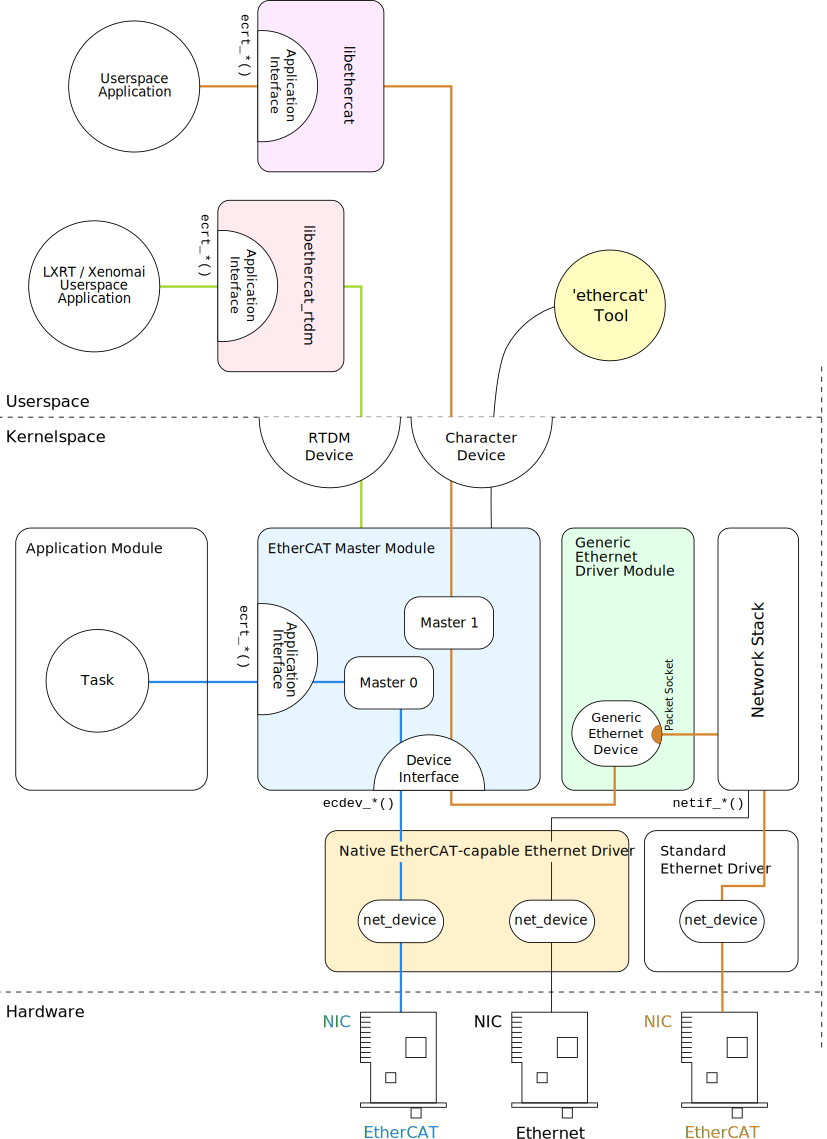
\includegraphics[width=\textwidth]{images/architecture}
  \caption{Architecture du ma\^itre}
  \label{fig:arch}
\end{figure}

Les composants de l'environnement du ma\^itre sont d\'ecrits
ci-dessous:

\begin{description}

\item[Master Module]\index{Master Module} Module noyau contenant une
  ou plusieurs instances du ma\^itre EtherCAT (voir
  \autoref{sec:mastermod}), le ``Device Interface'' (interface du
  p\'eriph\'erique, voir \autoref{sec:ecdev}) et l'``Application
  Interface'' (interface de programmation applicative, voir
  \autoref{chap:api}).

\item[Device Modules]\index{Device modules} Modules\index{Device
  modules} de pilotes de p\'eriph\'erique Ethernet supportant EtherCAT
  qui offrent leurs p\'eriph\'eriques au ma\^itre EtherCAT via
  l'interface du p\'eriph\'erique (voir \autoref{sec:ecdev}).  Ces
  pilotes r\'eseaux modifi\'es peuvent g\'erer en parall\`ele les
  interfaces r\'eseaux utilis\'ees pour les op\'erations EtherCAT et
  les interfaces r\'eseaux Ethernet ``normales''.  Un ma\^itre peut
  accepter un p\'eriph\'erique particulier pour envoyer et recevoir
  des trames EtherCAT. Les p\'eriph\'eriques Ethernet d\'eclin\'es
  par le module ma\^itre sont connect\'es comme d'habitude \`a la pile
  r\'eseau du noyau.

\item[Application]\index{Application} Un programme qui utilise le
  ma\^itre EtherCAT (habituellement pour un \'echange cyclique de
  donn\'ees de processus avec les esclaves EtherCAT).  Ces programmes
  n'appartiennent pas au code du ma\^itre EtherCAT\footnote{Toutefois,
  il y a des exemples fournis dans le dossier \textit{examples/}.},
  mais ils doivent \^etre g\'en\'er\'es ou \'ecrits par
  l'utilisateur. Une application peut demander un ma\^itre via l'API
  (voir \autoref{chap:api}). Si la demande r\'eussie, elle a alors le
  contr\^ole du ma\^itre: elle peut fournir une configuration de bus
  et \'echanger des donn\'ees de processus. Les applications peuvent
  \^etre des modules noyaux (qui utilisent directement l'API du noyau)
  ou des programmes dans l'espace utilisateur, qui utilisent l'API via
  la biblioth\`eque EtherCAT (voir~\autoref{sec:userlib}), ou la
  biblioth\`eque RTDM (voir~\autoref{sec:rtdm}).

\end{description}

%------------------------------------------------------------------------------

\section{Module Ma\^itre}
\label{sec:mastermod}
\index{Master module}

Le module noyau du ma\^itre EtherCAT \textit{ec\_master} peut contenir
plusieurs instances ma\^itresses. Chaque ma\^itre attend des
p\'eriph\'eriques Ethernet particuliers identifi\'es par leurs adresses
MAC\index{MAC address}. Ces adresses doivent \^etre sp\'ecifi\'ees au
chargement du module via le param\`etre de module
\textit{main\_devices} (et en option: \textit{backup\_devices}). Le
nombre d'instances ma\^itresses \`a initialiser est d\'efini par le
nombre d'adresses MAC fournies.

La commande ci-dessous charge le module ma\^itre avec une unique
instance ma\^itresse qui attend un seul p\'eriph\'erique Ethernet dont
l'adresse MAC est \lstinline+00:0E:0C:DA:A2:20+. Le ma\^itre sera
accessible \`a l'index $0$.

\begin{lstlisting}
# `\textbf{modprobe ec\_master main\_devices=00:0E:0C:DA:A2:20}`
\end{lstlisting}

Pour plusieurs ma\^itres, des virgules s\'eparent les adresses MAC :

\begin{lstlisting}
# `\textbf{modprobe ec\_master main\_devices=00:0E:0C:DA:A2:20,00:e0:81:71:d5:1c}`
\end{lstlisting}

Les deux ma\^itres peuvent \^etre adress\'es par leurs indices
respectifs 0 et 1 (voir \autoref{fig:masters}). L'index du ma\^itre
est requis par la fonction \lstinline+ecrt_master_request()+ de l'API
(voir \autoref{chap:api}) et par l'option \lstinline+--master+ de
l'outil de commande en ligne \textit{ethercat} (voir
\autoref{sec:tool}), qui vaut $0$ par d\'efaut.

\begin{figure}[htbp]
  \centering
  \includegraphics[width=.5\textwidth]{images/masters}
  \caption{Plusieurs ma\^itres dans un module}
  \label{fig:masters}
\end{figure}

\paragraph{Niveau de d\'everminage} Le module ma\^itre a aussi un
param\`etre \textit{debug\_level} pour configurer le niveau initial de
d\'everminage pour tous les ma\^itres (voir
aussi~\autoref{sec:ethercat-debug}).

\paragraph{Script d'initialisation}
\index{Init script}

Dans la plupart des cas, il n'est pas n\'ecessaire de charger
manuellement le module ma\^itre et les modules des pilotes Ethernet.
Un script d'initialisation est disponible pour d\'emarrer le ma\^itre
en tant que service (voir \autoref{sec:system}). Un fichier de service
est aussi disponible pour les syst\`emes qui sont g\'er\'es par
systemd \cite{systemd}.

\paragraph{Syslog}

Le module ma\^itre publie des informations \`a propos de son \'etat et ses
\'ev\'enement dans le tampon circulaire du noyau. Elles aboutissent aussi
dans les journaux syst\`emes. La commande de chargement du module
devrait produire les messages ci-dessous:

\begin{lstlisting}
# `\textbf{dmesg | tail -2}`
EtherCAT: Master driver `\masterversion`
EtherCAT: 2 masters waiting for devices.

# `\textbf{tail -2 /var/log/messages}`
Jul  4 10:22:45 ethercat kernel: EtherCAT: Master driver `\masterversion`
Jul  4 10:22:45 ethercat kernel: EtherCAT: 2 masters waiting
                                 for devices.
\end{lstlisting}

Les messages du ma\^itre sont pr\'efix\'es par \lstinline+EtherCAT+ pour
faciliter la recherche dans les journaux.

%------------------------------------------------------------------------------

\section{Phases du ma\^itre}
\index{Master phases}

Chaque ma\^itre EtherCAT fourni par le module ma\^itre (voir
\autoref{sec:mastermod}) traverse plusieurs phases au cours de son
ex\'ecution (voir \autoref{fig:phases}):

\begin{figure}[htbp]
  \centering
  \includegraphics[width=.9\textwidth]{images/phases}
  \caption{Phases et transitions du ma\^itre}
  \label{fig:phases}
\end{figure}

\begin{description}

\item[Phase orpheline (Orphaned)]\index{Orphaned phase} Ce mode prend
  effet quand le ma\^itre attend encore pour se connecter \`a ses
  p\'eriph\'eriques Ethernet. Aucune communication de bus n'est possible
  pour l'instant.

\item[Phase paresseuse (Idle)]\index{Idle phase} Ce mode prend effet
  quand le ma\^itre a accept\'e tous les p\'eriph\'eriques Ethernet
  requis, mais qu'aucune application ne l'a encore mobilis\'e. Le
  ma\^itre ex\'ecute son automate (voir \autoref{sec:fsm-master}), qui
  analyse automatiquement le bus pour rechercher les esclaves et
  ex\'ecuter les op\'erations en attente depuis l'interface en espace
  utilisateur (par exemple les acc\`es SDO).  L'outil en ligne de
  commande peut \^etre utilis\'e pour acc\'eder au bus, mais il n'y a
  aucun \'echange de donn\'ee de processus parce que la configuration
  du bus est manquante.

\item[Phase d'op\'eration]\index{Operation phase} Le ma\^itre est
  mobilis\'e par une application qui peut fournir une configuration de
  bus et \'echanger des donn\'ees de processus..

\end{description}

%------------------------------------------------------------------------------

\section{Donn\'ees de processus}
\label{sec:processdata}

Cette section pr\'esente quelques termes et id\'ees sur la mani\`ere
dont le ma\^itre traite les donn\'ees de processus.

\paragraph{Image des donn\'ees de processus}
\index{Process data}

Les esclaves pr\'esentent leurs entr\'es et sorties au ma\^itre au
travers d'objet de donn\'ees de processus ``Process Data Objects''
(PDOs\index{PDO}). Les PDOs disponibles peuvent \^etre d\'etermin\'es
en lisant les cat\'egories SII TxPDO et RxPDO de l'esclave depuis
l'E$^2$PROM (en cas de PDOs fixes) ou en lisant les objets CoE
appropri\'es (voir \autoref{sec:coe}), si disponibles. L'application
peut inscrire les entr\'ees des PDOs pour l'\'echange pendant
l'op\'eration cyclique.  La somme de toutes les entr\'ees PDO
inscrites d\'efinit l'``image des donn\'ees du processus'', qui peut
\^etre \'echang\'ee via des datagrammes avec des acc\`es m\'emoires
``logiques'' (comme LWR\footnote{LWR: Logical Write},
LRD\footnote{LRD: Logical Read} ou LRW\footnote{LRW: Logical
Read/Write}) pr\'esent\'es dans ~\cite[sec.~5.4]{dlspec}.

\paragraph{Domaine de donn\'ees de processus}
\index{Domain}

Les images des donn\'ees de processus peuvent \^etre facilement
g\'er\'ees en cr\'eant des ``domaines'', qui permettent l'\'echange de
PDO group\'es. Ils s'occupent \'egalement de g\'erer les structures
des datagrammes qui sont n\'ecessaires pour \'echanger les PDOs.  Les
domaines sont obligatoires pour l'\'echange de donn\'ees de processus,
donc il doit y en avoir au moins un. Ils ont \'et\'e introduits pour
les raisons suivantes:

\begin{itemize}

\item La taille maximale d'un datagramme est limit\'ee par celle d'une
  trame Ethernet. La taille maximale des donn\'ees est la taille du
  champ ``donn\'ees'' d'Ethernet moins l'ent\^ete de la trame
  Ethernet, moins l'ent\^ete du datagramme EtherCAT et moins la
  terminaison du datagramme EtherCAT: $1500 - 2 - 12 - 2 = 1484$
  octets. Si la taille de l'image des donn\'ees de processus d\'epasse
  cette limite, il faut envoyer plusieurs trames et partitionner
  l'image pour utiliser plusieurs datagrammes. Un domaine g\`ere cela
  automatiquement.

\item Tous les PDOs n'ont pas besoin d'\^etre \'echang\'es \`a la
  m\^eme fr\'equence: les valeurs des PDOs peuvent varier lentement au
  cours du temps (par exemple des valeurs de temp\'erature), aussi les
  \'echanger \`a haute fr\'equence serait un gaspillage de la bande
  passante du bus. Pour cette raison, plusieurs domaines peuvent
  \^etre cr\'e\'es, pour grouper diff\'erents PDOs et ainsi s\'eparer
  les \'echanges.

\end{itemize}

Il n'y a aucune limite sup\'erieure pour le nombre de domaines, mais
chaque domaine occupe une FMMU\footnote{FMMU: Fieldbus Memory
Management Unit} dans l'esclave concern\'e, donc le nombre maximal de
domaines est en fait limit\'e par les esclaves.

\paragraph{Configuration FMMU}
\index{FMMU!Configuration}

Une application peut inscrire des entr\'ees PDO pour l'\'echange.
Chaque entr\'ee PDO et son PDO parent font partie d'une zone m\'emoire
dans la m\'emoire physique de l'esclave, qui est prot\'eg\'ee par un
gestionnaire de synchronisation (sync manager) \cite[sec.~6.7]{dlspec}
pour des acc\`es synchronis\'es.  Pour que le gestionnaire de
synchronisation r\'eagisse \`a un datagramme qui acc\`ede \`a sa
m\'emoire, il est n\'ecessaire d'acc\'eder au dernier octet couvert
par le gestionnaire de synchronisation. Sinon le gestionnaire de
synchronisation ne r\'eagira pas au datagramme et aucune donn\'ee ne
sera \'echang\'ee.  C'est pourquoi l'ensemble de la zone m\'emoire
synchronis\'ee doit \^etre inclus dans l'image des donn\'ees de
processus: par exemple; si une entr\'ee PDO particuli\`ere d'un
esclave est inscrite pour l'\'echange avec un domaine particulier, une
FMMU sera configur\'ee pour mapper toute la m\'emoire prot\'eg\'ee par
le gestionnaire de synchronisation dans laquelle l'entr\'ee PDO
r\'eside. Si une deuxi\`eme entr\'ee PDO du m\^eme esclave est
inscrite pour l'\'echange de donn\'ee de processus au sein du m\^eme
domaine, et s'il r\'eside dans la m\^eme zone m\'emoire prot\'eg\'ee
par le gestionnaire de synchronisation que la premi\`ere entr\'ee,
alors la configuration FMMU n'est pas modifi\'ee, parce que la
m\'emoire d\'esir\'ee fait d\'ej\`a partie de l'image des donn\'ees du
processus du domaine. Si la deuxi\`eme entr\'ee appartenait \`a une
autre zone prot\'eg\'ee par le gestionnaire de synchronisation, alors
cette zone enti\`ere serait aussi incluse dans l'image des donn\'ees
des processus des domaines.

\autoref{fig:fmmus} fournit un aper\c{c}u de la mani\`ere de
configurer les FMMUs pour mapper la m\'emoire physique vers les images
logiques des donn\'ees des processus.

\begin{figure}[htbp]
  \centering
  \includegraphics[width=\textwidth]{images/fmmus}
  \caption{Configuration FMMU}
  \label{fig:fmmus}
\end{figure}

%------------------------------------------------------------------------------

\chapter{Interface de Programmation Applicative (API)}
\label{chap:api}
\index{Application interface}

% TODO
%
% Interface version
% Master Requesting and Releasing
% Master Locking
% Configuring PDO assignment and mapping
% Domains (memory)
% PDO entry registration
% SDO configuration
% SDO access
% IDN configurations
% IDN access

L'interface de programmation applicative fournit les fonctions et
structures de donn\'ees pour acc\'eder au ma\^itre EtherCAT.  La
documentation compl\`ete de l'interface est incluse sous forme de
commentaires Doxygen~\cite{doxygen} dans le fichier d'ent\^ete
\textit{include/ecrt.h}. Elle peut \^etre lue directement depuis les
commentaires du fichier, ou plus confortablement sous forme de
documentation HTML. La g\'en\'eration du HTML est d\'ecrite dans
\autoref{sec:gendoc}.

Les sections suivantes couvrent une description g\'en\'erale de l'API.

Chaque application devrait utiliser le ma\^itre en deux \'etapes:

\begin{description}

\item[Configuration] Le ma\^itre est mobilis\'e et la configuration
  est appliqu\'ee. Par exemple, les domaines sont cr\'e\'es, les
  esclaves sont configur\'es et les entr\'ees PDO sont inscrites.
  (voir \autoref{sec:masterconfig}).

\item[Op\'eration] Le code cyclique est ex\'ecut\'e et les donn\'ees de
  processus sont \'echang\'ees (voir \autoref{sec:cyclic}).

\end{description}

\paragraph{Exemple d'Applications}\index{Example Applications}
Il y a quelques exemples d'applications dans le sous-dossier
\textit{examples/} du code du ma\^itre. Ils sont document\'es dans le
code source.

%------------------------------------------------------------------------------

\section{Configuration du ma\^itre}
\label{sec:masterconfig}

La configuration du bus est fournie via l'API. La
\autoref{fig:app-config} donne une vue d'ensemble des objets qui
peuvent \^etre configur\'es par l'application.

\begin{figure}[htbp]
  \centering
  \includegraphics[width=.8\textwidth]{images/app-config}
  \caption{Configuration du ma\^itre}
  \label{fig:app-config}
\end{figure}

\subsection{Configuration de l'esclave}

L'application doit dire au ma\^itre quelle est la topologie attendue
du bus.  Ceci peut \^etre fait en cr\'eant des ``configurations
d'esclaves''.  Une configuration d'esclave peut \^etre vue comme un
esclave attendu.  Quand une configuration d'esclave est cr\'e\'ee,
l'application fournit la position sur le bus (voir ci-dessous),
l'identifiant du fabricant (vendor id) et le code du produit (product
code).

Quand la configuration du bus est appliqu\'ee, le ma\^itre v\'erifie
s'il y a un esclave avec l'identifiant du fabricant et le code du
produit \`a la position donn\'ee.  Si c'est le cas, la configuration
de l'esclave est ``attach\'ee'' \`a l'esclave r\'eel sur le bus et
l'esclave est configur\'e en fonction des param\`etres fournis par
l'application.  L'\'etat de la configuration de l'esclave peut soit
\^etre demand\'e via l'API ou via l'outil en ligne de commande (voir
\autoref{sec:ethercat-config}).

\paragraph{Position de l'esclave} La position de l'esclave doit \^etre
sp\'ecifi\'ee sous forme d'un couple ``alias'' et ``position''.  Ceci
permet d'adresser les esclaves via la position absolue sur le bus ou
via un identifiant stock\'e et appel\'e ``alias'' ou via un m\'elange
des deux.  L'alias est une valeur 16 bits stock\'ee dans E$^2$PROM de
l'esclave.  Il peut \^etre modifi\'e via l'outil en ligne de commande
(voir \autoref{sec:ethercat-alias}).  \autoref{tab:slaveposition}
montre comment les valeurs sont interpr\'et\'ees.

\begin{table}[htbp]
  \centering
  \caption{Sp\'ecifier la position d'un esclave}
  \label{tab:slaveposition}
  \vspace{2mm}
  \begin{tabular}{c|c|p{70mm}}
    Alias & Position & Interpr\'etation\\
    \hline

    \lstinline+0+ & \lstinline+0+ -- \lstinline+65535+ &

    Adressage par position. Le param\`etre de position est
    interpr\'et\'e comme la position absolue de l'anneau sur le
    bus.\\ \hline

    \lstinline+1+ -- \lstinline+65535+ & \lstinline+0+ -- \lstinline+65535+ &

    Adressage par alias. Le param\`etre de position est interpr\'et\'e
    comme une position relative apr\`es le premier esclave
    avec une adresse d'alias donn\'ee. \\ \hline

  \end{tabular}
\end{table}

\autoref{fig:attach} montre un exemple d'attachement des
configurations des esclaves. Certaines configurations sont
attach\'ees, tandis que d'autres restes d\'etach\'ees. La liste
ci-dessous en donne les raisons en commen\c{c}ant par la configuration
de l'esclave du haut.

\begin{figure}[htbp]
  \centering
  \includegraphics[width=.7\textwidth]{images/attach}
  \caption{Attachement de la configuration des esclaves}
  \label{fig:attach}
\end{figure}

\begin{enumerate}

\item L'alias z\'ero signifie un adressage simple par position.
  L'esclave \#1 existe et l'identifiant du fabricant et le code
  produit correspondent aux valeurs attendues.

\item Bien que l'esclave en position 0 a \'et\'e trouv\'e, le code
  produit ne correspond pas, aussi la configuration n'est pas
  attach\'ee.

\item L'alias n'est pas z\'ero, aussi l'adressage par alias est
  utilis\'e.  L'esclave \#2 est le premier esclave avec l'alias
  \lstinline+0x2000+. Comme la valeur de position est z\'ero, le
  m\^eme esclave est utilis\'e.

\item Il n'y a aucun esclave avec l'alias demand\'e, aussi la
  configuration ne peut pas \^etre attach\'ee.

\item L'esclave \#2 est encore le premier esclave avec l'alias
  \lstinline+0x2000+, mais la position est maintenant 1, aussi
  l'esclave \#3 est attach\'e.
\end{enumerate}

Si les sources du ma\^itre sont configur\'ees avec
\lstinline+--enable-wildcards+, alors
\lstinline+0xffffffff+ correspond \`a n'importe quel identifiant de fabricant et/ou code produit.

%------------------------------------------------------------------------------

\section{Op\'eration cyclique}
\label{sec:cyclic}

Pour entrer dans le mode d'op\'eration cyclique, le ma\^itre doit \^etre
``activ\'e'' pour calculer l'image des donn\'ees de processus et appliquer
la configuration du bus pour la premi\`ere fois. Apr\`es l'activation,
l'application est responsable d'envoyer et recevoir les trames.
La configuration ne peut pas \^etre modifi\'ee apr\`es l'activation.

% TODO
%
% PDO endianess
% Datagram injection

%------------------------------------------------------------------------------

\section{Gestionnaires VoE}
\label{sec:api-voe}

Pendant la phase de configuration, l'application peut cr\'eer des
gestionnaires pour le protocole de bo\^ite aux lettres VoE, d\'ecrit
dans \autoref{sec:voe}. Un gestionnaire VoE appartient toujours \`a
une configuration d'esclave particuli\`ere, aussi la fonction de
cr\'eation est une m\'ethode de la configuration de l'esclave.

Un gestionnaire VoE g\`ere les donn\'ees VoE et les datagrammes
utilis\'es pour transmettre et recevoir les messages VoE. Il contient
l'automate n\'ecessaire au transfert des messages VoE.

L'automate VoE peut traiter seulement une op\'eration \`a la fois. Par
cons\'equent, seule une op\'eration de lecture ou une op\'eration
d'\'ecriture peut \^etre \'emise \`a un moment donn\'e\footnote{Si, on
d\'esire envoyer et recevoir simutan\'ement, deux gestionnaires VoE
peuvent \^etre cr\'e\'es pour la configuration de l'esclave.}. Apr\`es
l'initialisation de l'op\'eration, le gestionnaire doit \^etre
ex\'ecut\'e de mani\`ere cyclique jusqu'\`a ce qu'il se termine.
Apr\`es cela, les r\'esultats de l'op\'eration peuvent \^etre
r\'ecup\'er\'es.

Un gestionnaire VoE a sa propre structure de datagramme, qui est
marqu\'e pour l'\'echange apr\`es chaque pas d'ex\'ecution. Aussi,
l'application peut d\'ecider, combien de gestionnaires elle ex\'ecute
avant d'envoyer les trames EtherCAT correspondantes.

Pour obtenir davantage d'information sur les gestionnaires VoE,
consultez la documentation des fonctions de l'API et les exemples
d'applications fournis dans le dossier \textit{examples/}.

%------------------------------------------------------------------------------

\section{Acc\`es concurrents au ma\^itre}
\label{sec:concurr}
\index{Concurrency}

Dans certains cas,  plusieurs instances utilisent un seul ma\^itre,
par exemple quand une application \'echange des donn\'ees de processus
cyclique et qu'il y a des esclaves EoE qui ont besoin d'\'echanger des
donn\'ees Ethernet avec le noyau (voir \autoref{sec:eoe}). Pour
cette raison, le ma\^itre est une ressource partag\'ee qui doit \^etre
s\'equentialis\'ee. Ceci est habituellement r\'ealis\'e en
verrouillant au moyen de s\'emaphores ou d'autres m\'ethodes pour
prot\'eger les sections critiques.

Le ma\^itre ne fournit pas lui-m\^eme de m\'ecanismes de
verrouillage, parce qu'il ne peut conna\^itre le type de
verrou appropri\'e. Par exemple, si l'application est en espace noyau
et utilise la fonctionnalit\'e RTAI, les s\'emaphores ordinaires du
noyau ne seraient pas suffisants. Pour cela, une d\'ecision de
conception importante a \'et\'e faite: l'application qui a r\'eserv\'e
un ma\^itre doit en avoir le contr\^ole total, c'est pourquoi elle
doit prendre la responsabilit\'e de fournir les m\'ecanismes de
verrouillage appropri\'es.  Si une autre instance veut acc\'eder au
ma\^itre, elle doit demander l'acc\`es au bus via des fonctions de
rappels qui doivent \^etre fournis par l'application.  De plus,
l'application peut refuser l'acc\`es au ma\^itre, si elle consid\`ere
que le moment est g\^enant.

\begin{figure}[htbp]
  \centering
  \includegraphics[width=.6\textwidth]{images/master-locks}
  \caption{Acc\`es concurrent au ma\^itre}
  \label{fig:locks}
\end{figure}

L'exemple \autoref{fig:locks} montre comment deux processus partagent
un ma\^itre: la t\^ache cyclique de l'application utilise le ma\^itre
pour l'\'echange de donn\'ees de processus, tandis que le processus
EoE interne au ma\^itre l'utilise pour communiquer avec les esclaves
EoE.  Les deux ont acc\`es au bus de temps en temps, mais le processus
EoE le fait en ``demandant'' \`a l'application de r\'ealiser l'acc\`es
au bus pour lui.  De cette mani\`ere, l'application peut utiliser le
m\'ecanisme de verrouillage appropri\'e pour \'eviter d'acc\`eder au
bus en m\^eme temps.  Voir la documentation de l'API
(\autoref{chap:api}) pour savoir comment utiliser ces fonctions de
rappel.

%------------------------------------------------------------------------------

\section{Horloges distribu\'ees}
\label{sec:dc}
\index{Distributed Clocks}

\`A partir de la version 1.5, le ma\^itre supporte les ``horloges distribu\'ees'' (Distributed Clocks) EtherCAT pour synchroniser les horloges des esclaves
sur le bus avec l'horloge de ``r\'ef\'erence''
(qui est l'horloge locale du premier esclave qui supporte l'horloge
distribu\'ee) et pour synchroniser l'horloge de r\'ef\'erence avec
``l'horloge ma\^itresse'' (qui est l'horloge locale du ma\^itre).
Toutes les autres horloges du bus (apr\`es l'horloge de r\'ef\'erence)
sont consid\'er\'es comme ``horloges esclaves'' (voir \autoref{fig:dc}).

\begin{figure}[htbp]
  \centering
  \includegraphics[width=.8\textwidth]{images/dc}
  \caption{Horloges distribu\'ees}
  \label{fig:dc}
\end{figure}

\paragraph{Horloges locales} Tout esclave EtherCAT qui supporte
l'horloge distribu\'ee
poss\`ede un registre d'horloge locale avec une r\'esolution \`a la
nanoseconde.  Si l'esclave est allum\'e, l'horloge d\'emarre depuis
z\'ero, ce qui signifie que lorsque des esclaves sont allum\'es \`a
diff\'erents instants, leurs horloges auront des valeurs diff\'erentes.
Ces ``d\'ecalages'' doivent \^etre compens\'es par le m\'ecanisme des
horloges distribu\'ees.  En outre, les horloges ne tournent
pas exactement \`a la m\^eme vitesse, puisque les quartzs ont une
d\'eviation de leur fr\'equence naturelle.  Cette d\'eviation est
habituellement tr\`es faible, mais au bout de longues p\'eriodes,
l'erreur s'accumulera et la diff\'erence entre les horloges locales
grandira. Cette ``d\'erive'' des horloges doit aussi \^etre
compens\'ee par le m\'ecanisme des horloges distribu\'ees.

\paragraph{Temps de l'Application} La base de temps commune pour le bus
doit \^etre fournie par l'application.
Ce temps d'application $t_\text{app}$ est utilis\'e

\begin{enumerate}
\item pour configurer les d\'ecalages des horloges des esclaves (voir ci-dessous),
\item pour programmer les temps de d\'emarrage de l'esclave pour
  la g\'en\'eration des impulsions synchrones. (voir ci-dessous)
\item pour synchroniser les horloges de r\'ef\'erence avec l'horloge
  ma\^itresse (optionnel).
\end{enumerate}

\paragraph{Compensation du d\'ecalage} Pour la compensation du d\'ecalage,
chaque esclave fournit un registre de ``d\'ecalage du temps
syst\`eme'' $t_\text{off}$, qui est ajout\'e \`a la valeur de
l'horloge interne $t_\text{int}$ pour obtenir le ``Temps Syst\`eme''
$t_\text{sys}$:

\begin{eqnarray}
t_\text{sys} & = & t_\text{int} + t_\text{off} \\
\Rightarrow t_\text{int} & = & t_\text{sys} - t_\text{off} \nonumber
\end{eqnarray}

Le ma\^itre lit les valeurs des deux registres pour calculer un nouveau
d\'ecalage du temps syst\`eme de telle mani\`ere que
le temps syst\`eme r\'esultant corresponde au temps de l'application du
ma\^itre $t_\text{app}$:

\begin{eqnarray}
t_\text{sys} & \stackrel{!}{=} & t_\text{app} \\
\Rightarrow t_\text{int} + t_\text{off} & \stackrel{!}{=} & t_\text{app} \nonumber \\
\Rightarrow t_\text{off} & = & t_\text{app} - t_\text{int} \nonumber \\
\Rightarrow t_\text{off} & = & t_\text{app} - (t_\text{sys} - t_\text{off}) \nonumber \\
\Rightarrow t_\text{off} & = & t_\text{app} - t_\text{sys} + t_\text{off}
\end{eqnarray}


La petite erreur de d\'ecalage du temps r\'esultant des diff\'erences
de temps entre la lecture et l'\'ecriture des registres sera compens\'ee
par la compensation de la d\'erive.

\paragraph{Compensation de la d\'erive} La compensation de la d\'erive
est possible gr\^ace \`a un m\'ecanisme sp\'ecial de chaque esclave
compatible avec les horloges distribu\'ees: une op\'eration
d'\'ecriture dans le registre du ``Temps syst\`eme'' obligera la boucle
de contr\^ole du temps interne \`a comparer le temps \'ecrit (moins le
d\'elai de transmission programm\'e, voir ci-dessous) avec le temps
syst\`eme courant.  L'erreur de temps calcul\'ee sera utilis\'ee comme
une entr\'ee pour le contr\^oleur de temps, qui ajustera la vitesse de
l'horloge locale pour \^etre l\'eg\`erement plus rapide ou plus
lente\footnote{ L'horloge locale de l'esclave sera incr\'ement\'ee de
\unit{9}{\nano\second}, \unit{10}{\nano\second} ou
\unit{11}{\nano\second} toute les \unit{10}{\nano\second}.}, en
fonction du signe de l'erreur.

\paragraph{D\'elais de transmission} La trame Ethernet a besoin
d'une petite quantit\'e de temps pour se propager d'esclave en
esclave.  Les d\'elais de transmission s'accumulent sur le bus et
peuvent attendre la magnitude de la microseconde et doivent alors
\^etre pris en compte par la compensation de la d\'erive.  Les
esclaves EtherCAT qui supportent les horloges distribu\'ees
fournissent un m\'ecanisme pour mesurer les d\'elais de transmission:
pour chacun des 4 ports de l'esclave il y a un registre d'heure de
r\'eception.  Une op\'eration d'\'ecriture sur le registre d'heure de
r\'eception du port d\'emarre la mesure et l'heure syst\`eme courante
est captur\'ee et stock\'ee dans un registre d'heure de r\'eception
une fois que la trame est re\c{c}ue sur le port correspondant.  Le
ma\^itre peut lire le temps de r\'eception relatif puis calculer les
d\'elais entre les esclaves (en utilisant sa connaissance de la
topologie du bus), et finalement calculer les d\'elais de chaque
esclave avec l'horloge de r\'ef\'erence.  Ces valeurs sont
programm\'ees dans les registres de d\'elai de transmission des
esclaves. De cette mani\`ere, la compensation de la d\'erive peut
attendre une synchronie \`a la nanoseconde.

\paragraph{V\'erification de la synchronie}
Les esclaves compatibles avec les horloge distribu\'ees fournissent un
registre 32 bits ``Diff\'erence de l'heure syst\`eme'' \`a l'adresse
\lstinline+0x092c+, dans lequel la diff\'erence de temps syst\`eme de
la derni\`ere compensation de la d\'erive est stock\'ee avec une
r\'esolution d'une nanoseconde et un codage
signe-et-magnitude\footnote{Ceci permet une lecture-diffusion de tous
les registres de diff\'erence de temps syst\`eme sur le bus pour
obtenir une approximation de la valeur sup\'erieure.}. Pour v\'erifier
la synchronie du bus, les registres de diff\'erence du temps syst\`eme
peuvent aussi \^etre lus via l'outil en ligne de commande (voir
\autoref{sec:regaccess}):

\begin{lstlisting}
$ `\textbf{watch -n0 "ethercat reg\_read -p4 -tsm32 0x92c"}`
\end{lstlisting}

\paragraph{Signaux synchrones} Les horloge synchrones
sont seulement un pr\'e-requis pour des \'ev\`enements synchrones sur
le bus.  Chaque esclave qui supporte les horloges distribu\'ees
fournit deux ``signaux synchrones'', qui peuvent \^etre programm\'es
pour cr\'eer des \'ev\`enements, qui vont par exemple obliger
l'application esclave \`a capturer ses entr\'ees \`a un instant
pr\'ecis.  Un \'ev\`enement synchrone peut \^etre g\'en\'er\'e soit
une seule fois ou p\'eriodiquement, selon ce qui a du sens pour
l'application esclave.  La programmation des signaux synchrones est
une question de r\'eglage du mot ``AssignActivate'' et des temps
de cycle et d\'ecalage des signaux de synchronisation. Le mot
AssignActivate est sp\'ecifique \`a chaque esclave et doit \^etre
r\'ecup\'er\'e depuis la description XML de l'esclave
(\lstinline+Device+ $\rightarrow$ \lstinline+Dc+), o\`u se trouvent
aussi typiquement les signaux de configurations ``OpModes''.

%------------------------------------------------------------------------------

\chapter{Interfaces Ethernet}
\label{sec:devices}

Le protocole EtherCAT est fond\'e sur le standard Ethernet standard,
aussi un ma\^itre d\'epend du mat\'eriel Ethernet standard pour communiquer
avec le bus.

Le terme \textit{device} est utilis\'e comme synonyme pour mat\'eriel
d'interface r\'eseau Ethernet.

\paragraph{Pilotes natifs pour p\'eriph\'eriques Ethernet}
Il y a des modules natifs pour les pilotes de p\'eriph\'eriques (voir
\autoref{sec:native-drivers}) qui g\`erent le mat\'eriel Ethernet
qu'utilise le ma\^itre pour se connecter au bus EtherCAT. Ils offrent
leurs mat\'eriels Ethernet au module ma\^itre via l'interface de
device (voir \autoref{sec:ecdev}) et doivent \^etre capable de
pr\'eparer les p\'eriph\'eriques Ethernet pour les op\'erations
EtherCAT (temps r\'eel) ou pour les op\'erations ``normales'' en
utilisant la pile r\'eseau du noyau. L'avantage de cete approche est
que le ma\^itre peut op\'erer pratiquement directement avec le
mat\'eriel ce qui permet des performances
\'elev\'ees. L'inconv\'enient est qu'il faut avoir une version
compatible EtherCAT du pilote Ethernet original.

\paragraph{Pilote g\'en\'erique pour les p\'eriph\'eriques Ethernet}
\`A partir du ma\^itre version 1.5, il y a un module de pilote
g\'en\'erique pour les p\'eriph\'eriques Ethernet (voir
\autoref{sec:generic-driver}), qui utilise les couches basses de la
pile r\'eseau pour se connecter au mat\'eriel. L'avantage est que
n'importe quel p\'eriph\'erique Ethernet peut \^etre utilis\'e pour les
op\'erations EtherCAT, ind\'ependamment du pilote mat\'eriel r\'eel
(ainsi tous les pilotes Ethernet Linux sont support\'es sans
modification). L'inconv\'enient est que cette approche ne supporte
pas les extensions temps r\'eel, comme RTAI, parce que la pile
r\'eseau de Linux est utilis\'ee. Cependant la performance est
l\'eg\`erement moins bonne qu'avec l'approche native, car les donn\'ees
de la trame Ethernet doivent traverser la pile r\'eseau.

%------------------------------------------------------------------------------

\section{Principes de base du pilote r\'eseau}
\label{sec:networkdrivers}
\index{Network drivers}

EtherCAT repose sur le mat\'eriel Ethernet et le ma\^itre a besoin d'un
p\'eriph\'erique Ethernet physique pour communiquer avec le bus.
C'est pourquoi, il est n\'ecessaire de comprendre comment Linux g\`ere
les p\'eriph\'eriques r\'eseaux et leurs pilotes.

\paragraph{T\^aches d'un pilote r\'eseau}
Les pilotes de p\'eriph\'eriques r\'eseaux g\`erent habituellement les
deux couches les plus basses du mod\`ele OSI, qui sont la couche
physique et la couche liaison de donn\'ees.  Le p\'eriph\'erique
r\'eseau g\`ere nativement les probl\`emes de la couche physique: il
repr\'esente le mat\'eriel pour se connecter au m\'edia et pour
envoyer et recevoir des donn\'ees de la mani\`ere d\'ecrite par le
protocole de la couche physique.  Le pilote de p\'eriph\'erique
r\'eseau est responsable de r\'ecup\'erer les donn\'ees depuis la pile
r\'eseau du noyau et de les faire suivre au p\'eriph\'erique qui fait
la transmission physique.  Si des donn\'ees sont re\c{c}ues par le
p\'eriph\'erique alors le pilote est notifi\'e (habituellement au moyen
d'une interruption) et il doit lire les donn\'ees depuis la m\'emoire
du p\'eriph\'erique et l'envoyer \`a la pile r\'eseau.  Un pilote de
p\'eriph\'erique r\'eseau doit aussi g\'erer d'autres t\^aches telles
que le contr\^ole de la file d'attente, les statistiques et les
fonctionnalit\'es sp\'ecifiques du p\'eriph\'erique.

\paragraph{D\'emarrage du pilote} Habituellement, un pilote recherche
des p\'eriph\'eriques compatibles lors du chargement du module.  Pour
les pilotes PCI, ceci est fait en analysant le bus PCI et en
v\'erifiant les identifiants (ID) des p\'eriph\'eriques.  Si un
p\'eriph\'erique est trouv\'e, les structures de donn\'ees sont
allou\'ees et le p\'eriph\'erique est mis en service.

\paragraph{Fonctionnement des interruptions}\index{Interrupt} Un
p\'eriph\'erique r\'eseau fournit g\'en\'eralement une interruption
mat\'erielle qui est utilis\'ee pour notifier le pilote des trames
re\c{c}ues et des succ\`es ou erreurs des transmissions. Le pilote
doit enregistrer une routine de service d'interruption -- en anglais
\textit{interrupt service routine} --
(ISR\index{ISR}\nomenclature{ISR}{Interrupt Service Routine}), qui est
ex\'ecut\'ee \`a chaque fois que le mat\'eriel signale un tel
\'ev\`enement.  Si l'interruption a \'et\'e envoy\'ee par le bon
p\'eriph\'erique (plusieurs p\'eriph\'eriques peuvent partager une
m\^eme interruption mat\'erielle), la raison de l'interruption doit
\^etre d\'etermin\'ee en lisant le registre d'interruption du
p\'eriph\'erique.  Par exemple, si le drapeau pour les trames
re\c{c}ues est activ\'e, les donn\'ees des trames doivent \^etre
copi\'ees depuis le mat\'eriel vers la m\'emoire du noyau puis
transmise \`a la pile r\'eseau.

\paragraph{La structure \lstinline+net_device+}\index{net\_device} Le
pilote enregistre une structure \lstinline+net_device+ pour chaque
p\'eriph\'erique pour communiquer avec la pile r\'eseau et cr\'e\'e
une ``interface r\'eseau''.  Dans le cas d'un pilote Ethernet, cette
interface appara\^it sous la forme \textit{ethX}, o\`u X est le
num\'ero assign\'e par le noyau \`a l'enregistrement. La structure
\lstinline+net_device+ re\c{c}oit les \'ev\`enements (soit depuis
l'espace utilisateur, soit depuis la pile r\'eseau) via diff\'erentes
fonctions de rappel, qui doivent \^etre d\'efinies avant
l'enregistrement.  Toutes les fonctions de rappel ne sont pas
obligatoires, mais pour un fonctionnement raisonnable, celles qui sont
d\'efinies ci-dessous sont n\'ecessaires dans tous les cas:

\newsavebox\boxopen
\sbox\boxopen{\lstinline+open()+}
\newsavebox\boxstop
\sbox\boxstop{\lstinline+stop()+}
\newsavebox\boxxmit
\sbox\boxxmit{\lstinline+hard_start_xmit()+}
\newsavebox\boxstats
\sbox\boxstats{\lstinline+get_stats()+}

\begin{description}

\item[\usebox\boxopen] Cette fonction est appel\'ee quand la
  communication a d\'emar\'e, par exemple apr\`es une commande
  \lstinline+ip link set ethX up+ depuis l'espace utilisateur. La
  r\'eception des trames doit \^etre activ\'ee par le pilote.

\item[\usebox\boxstop] Le but de cette fonction de rappel est de
  ``fermer'' le p\'eriph\'erique, c'est-\`a-dire faire en sorte que le
  mat\'eriel cesse de recevoir des trames.

\item[\usebox\boxxmit] Cette fonction est appel\'ee pour chaque trame
  qui a \'et\'e transmise.  La pile r\'eseau passe la trame sous la
  forme d'un pointeur vers une structure \lstinline+sk_buff+ (``socket
  buffer''\index{Socket buffer} -- tampon de socket -- voir ci-dessous),
  qui doit \^etre lib\'er\'ee apr\`es l'envoi.

\item[\usebox\boxstats] Cet appel doit retourner un pointeur vers la
  structure \lstinline+net_device_stats+, qui doit \^etre
  continuellement mise \`a jour avec les statistiques des trames. Cela
  signifie qu'\`a chaque fois qu'une trame est re\c{c}ue, envoy\'ee ou
  qu'une erreur se produit, le compteur appropri\'e de cette structure
  doit \^etre augment\'e.

\end{description}

L'inscription r\'eelle est faite par l'appel \lstinline+register_netdev()+,
la d\'esinscription est faite par \lstinline+unregister_netdev()+.

\paragraph{L'interface \lstinline+netif+}\index{netif} Toute autre
communication dans la direction interface $\to$ r\'eseau est faite via
les appels \lstinline+netif_*()+. Par exemple, apr\`es l'ouverture
r\'eussie du p\'eriph\'erique, la pile r\'eseau doit \^etre
notifi\'ee, pour qu'elle puisse maintenant passer les trames \`a
l'interface.  Ceci est fait en appelant
\lstinline+netif_start_queue()+. Apr\`es cet appel, la fonction de
rappel \lstinline+hard_start_xmit()+ peut \^etre rappel\'ee par la
pile r\'eseau. De plus, un pilote r\'eseau g\`ere habituellement une
file d'attente pour la transmission des trames.  Quand elle est pleine,
il faut informer la pile r\'eseau qu'elle doit cesser de pousser
davantage de trames pendant un moment.  Ceci se produit avec un appel
\`a \lstinline+netif_stop_queue()+. Si des trames ont \'et\'e
envoy\'ees, et qu'il y a \`a nouveau suffisamment de place pour les
mettre en file d'attente, ceci peut \^etre notifi\'e avec
\lstinline+netif_wake_queue()+. Un autre appel important est
\lstinline+netif_receive_skb()+\footnote{Cette fonction fait partie de
NAPI (``New API''), qui remplace la technique du noyau 2.4 pour
interfacer la pile r\'eseau (avec \lstinline+netif_rx()+). NAPI est
une technique pour am\'eliorer la performance r\'eseau de
Linux. Davantage d'information dans
\url{http://www.cyberus.ca/~hadi/usenix-paper.tgz}.}: il passe une
trame qui vient juste d'\^etre re\c{c}ue par le p\'eriph\'erique, \`a
la pile r\'eseau.  Les donn\'ees de la trame doivent \^etre incluses
\`a cet effet dans le ``tampon de socket'' (voir ci-dessous).

\paragraph{Tampons de Socket}\index{Socket buffer} Les tampons de sockets
sont le type de donn\'ees fondamental de toute la pile r\'eseau.  Ils
servent de container pour les donn\'ees r\'eseaux et sont capables
d'ajouter rapidement des donn\'ees au d\'ebut et \`a la fin, ou bien
de les retirer. C'est pourquoi, un tampon de socket consiste en un
tampon allou\'e et plusieurs pointeurs qui marquent le d\'ebut du
tampon (\lstinline+head+), le d\'ebut des donn\'ees data
(\lstinline+data+), la fin des donn\'ees (\lstinline+tail+) et la fin
du tampon (\lstinline+end+). De plus, un tampon de socket contient les
informations d'ent\^ete pour le r\'eseau et (en cas de donn\'ees
re\c{c}ue), un pointeur vers le \lstinline+net_device+, qui l'a
r\'eceptionn\'e.  Il existe des fonctions qui cr\'eent un tampon
socket (\lstinline+dev_alloc_skb()+), ajoutent des donn\'ees au
d\'ebut (\lstinline+skb_push()+) ou \`a la fin
(\lstinline+skb_put()+), suppriment des donn\'ees au d\'ebut
(\lstinline+skb_pull()+) ou \`a la fin (\lstinline+skb_trim()+), ou
suppriment le tampon (\lstinline+kfree_skb()+).  Un tampon socket est
pass\'e de couche en couche et il est lib\'er\'e par la couche qui
s'en sert en dernier. En cas d'envoi, la lib\'eration est faite par le
pilote r\'eseau.

%------------------------------------------------------------------------------

\section{Les pilotes natifs pour p\'eriph\'eriques EtherCAT}
\label{sec:native-drivers}

Il y a quelques conditions qui s'appliquent au mat\'eriel Ethernet
lorsqu'il est utilis\'e avec un pilote Ethernet natif avec les
fonctionnalit\'es EtherCAT.

\paragraph{Mat\'eriel d\'edi\'e} Pour des raisons de performances et
de temps r\'eel, le ma\^itre EtherCAT a besoin d'un acc\`es direct et
exclusif au mat\'eriel Ethernet. Cela implique que le p\'eriph\'erique
r\'eseau ne doit pas \^etre connect\'e \`a la pile r\'eseau du noyau
comme d'habitude, car le noyau essaierait de l'utiliser comme un
p\'eriph\'erique Ethernet ordinaire.

\paragraph{Op\'eration sans interruption}\index{Interrupt}
Les trames EtherCAT voyagent au travers de l'anneau logique EtherCAT
et sont alors renvoy\'ees au ma\^itre.  La communication est hautement
d\'eterministe: une trame est envoy\'ee et sera re\c{c}ue apr\`es un
temps constant, aussi il n'y pas besoin de notifier le pilote de la
r\'eception de la trame. \`A la place, le ma\^itre peut interroger le
mat\'eriel pour les trames re\c{c}ues, s'il s'attend \`a ce qu'elles
soient d\'ej\`a arriv\'ees.


La \autoref{fig:interrupt} montre deux flots de travail pour la
transmission et r\'eception cyclique de trames avec et sans
interruptions.

\begin{figure}[htbp]
  \centering
  \includegraphics[width=.9\textwidth]{images/interrupt}
  \caption{Op\'eration avec interruption versus Op\'eration sans interruption}
  \label{fig:interrupt}
\end{figure}

Dans le flux de travail de gauche, ``Op\'eration avec interruption'',
les donn\'ees venant du dernier cycle sont d'abord trait\'ees et une
nouvelle trame est assembl\'ee avec des nouveaux datagrammes, puis
elle est envoy\'ee.  Le travail cyclique est fait pout l'instant.
Plus tard, quand la trame est \`a nouveau re\c{c}ue par le mat\'eriel,
une interruption est d\'eclench\'ee et l'ISR est ex\'ecut\'ee.  L'ISR
va r\'ecup\'erer les donn\'ees de la trame depuis le mat\'eriel et
commencer la dissection de la trame: les datagrammes seront trait\'es,
et alors les donn\'ees seront pr\^etes pour le traitement dans le
prochain cycle.

Dans le flux de travail de droite, ``Op\'eration sans interruption'',
aucune interruption mat\'erielle n'est activ\'ee. \`A la place, le
ma\^itre va sonder le mat\'eriel en ex\'ecutant l'ISR. Si la trame a
\'et\'e re\c{c}ue entre temps, elle sera diss\'equ\'ee. La situation est
maintenant la m\^eme qu'au d\'ebut de flux de travail de gauche : les
donn\'ees re\c{c}ues sont trait\'ees et une nouvelle trame est
assembl\'ee et envoy\'ee. Il n'y a rien d'autre \`a faire pour le
reste du cycle.

L'op\'eration sans interruption est pr\'ef\'erable, parce que les
interruptions mat\'erielles ne sont pas propices \`a l'am\'elioration
du comportement temps r\'eel du pilote: leurs incidences
ind\'eterministes contribuent \`a augmenter la gigue. En outre, si une
extension temps r\'eel (comme RTAI) est utilis\'ee, un effort
suppl\'ementaire devra \^etre fait pour hi\'erarchiser les
interruptions.

\paragraph{P\'eriph\'eriques Ethernet et EtherCAT}
Un autre probl\`eme r\'eside dans la fa\c{c}on dont Linux g\`ere les
p\'eriph\'eriques du m\^eme type.  Par exemple, un pilote
PCI\nomenclature{PCI}{Peripheral Component Interconnect, Bus
  informatique} analyse le bus PCI pour chercher des p\'eriph\'eriques
qu'il peut g\'erer.  Alors, il s'enregistre lui-m\^eme comme pilote
responsable pour tous les p\'eriph\'eriques trouv\'es.  Le probl\`eme
est que l'on ne peut pas dire \`a un pilote non modifi\'e d'ignorer un
p\'eriph\'erique pour l'utiliser ult\'erieurement pour EtherCAT. Il
faut donc un moyen de g\'erer plusieurs p\'eriph\'eriques du m\^eme
type, l'un \'etant r\'eserv\'e \`a EtherCAT, tandis que l'autre est
trait\'e comme un p\'eriph\'erique Ethernet ordinaire.

Pour toutes ces raisons, l'auteur a d\'ecid\'e que la seule solution
acceptable \'etait de modifier les pilotes Ethernet standards de
mani\`ere \`a ce qu'ils conservent leurs fonctionnalit\'es normales,
tout en gagnant la possibilit\'e de traiter un ou plusieurs
p\'eriph\'eriques comme \'etant compatibles EtherCAT.

Les avantages de cette solution sont list\'es ci-dessous:

\begin{itemize}
\item Pas besoin de dire aux pilotes standards d'ignorer certains
  p\'eriph\'eriques.
\item Un seul pilote r\'eseau pour les p\'eriph\'eriques EtherCAT et
  non-EtherCAT.
\item Pas besoin d'impl\'ementer un pilote r\'eseau depuis z\'ero et
  de rencontrer des probl\`emes que les anciens d\'eveloppeurs ont
  d\'ej\`a r\'esolus.
\end{itemize}

L'approche choisie a les inconv\'enients suivants:

\begin{itemize}
\item Le pilote modifi\'e est plus compliqu\'e car il doit g\'erer les
  p\'eriph\'eriques EtherCAT et non-EtherCAT.
\item De nombreuses diff\'erenciations de cas suppl\'ementaires dans le
  code du pilote.
\item Les modifications et changements dans les pilotes standards
  doivent \^etre port\'es de temps en temps vers les versions compatibles
  EtherCAT.
\end{itemize}

%------------------------------------------------------------------------------

\section{Le pilote de p\'eriph\'erique EtherCAT g\'en\'erique}
\label{sec:generic-driver}

Puisqu'il existe des approches pour activer un fonctionnement en temps
r\'eel \cite{rt-preempt} du noyau Linux complet, il est possible
d'op\'erer sans impl\'ementation native des pilotes de
p\'eriph\'eriques Ethernet compatibles EtherCAT et d'utiliser la pile
r\'eseau \`a la place. La \autoref{fig:arch} pr\'esente le ``Module de
pilote Ethernet g\'en\'erique'', qui se connecte \`a des
p\'eriph\'eriques Ethernet locaux via la pile r\'eseau.  Le module
noyau se nomme \lstinline+ec_generic+ et il peut \^etre charg\'e
apr\`es le module ma\^itre comme un pilote Ethernet compatible
EtherCAT.

Le pilote de p\'eriph\'erique g\'en\'erique analyse la pile r\'eseau
\`a la recherche d'interfaces enregistr\'ees par les pilotes de
p\'eriph\'eriques Ethernet.  Il offre tous les p\'eriph\'eriques
possibles au ma\^itre EtherCAT. Si le ma\^itre accepte un
p\'eriph\'erique, le pilote g\'en\'erique cr\'ee un socket de paquet
(voir \lstinline+man 7 packet+) avec \lstinline+socket_type+ mis \`a
\lstinline+SOCK_RAW+, li\'e \`a ce p\'eriph\'erique.  Toutes les
fonctions de l'interface de ce p\'eriph\'erique (voir
\autoref{sec:ecdev}) op\'ereront alors sur ce socket.

Les avantages de cette solution sont list\'es ci-dessous:

\begin{itemize}
\item Tout mat\'eriel, qui est g\'er\'e par un pilote Ethernet
  Linux, peut \^etre utilis\'e pour EtherCAT.
\item Aucune modification n'est n\'ec\'essaire sur les pilotes Ethernet
  r\'eels.
\end{itemize}

L'approche g\'en\'erique a les inconv\'enients suivants:

\begin{itemize}
\item La performance est un peut moins bonne qu'avec l'approche
  native, parce que les donn\'ees de la trame doivent traverser les
  couches basses de la pile r\'eseau.
\item Il n'est pas possible d'utiliser des extensions en temps r\'eel
  dans le noyau comme RTAI avec le pilote g\'en\'erique, car le code
  de la pile r\'eseau utilise des allocations dynamiques de m\'emoire
  et d'autres choses, qui pourraient provoquer le gel du syst\`eme
  dans un contexte temps r\'eel.
\end{itemize}

\paragraph{Activation du p\'eriph\'erique} Dans le but d'envoyer
et recevoir des trames au travers d'un socket, le p\'eriph\'erique
Ethernet li\'e \`a ce socket doit \^etre activ\'e, autrement toutes
les trames seront rejet\'ees.  L'activation doit avoir lieu avant le
chargement du module ma\^itre et peut avoir lieu de diff\'erentes
mani\`eres:

\begin{itemize}

\item Ad-hoc, en utilisant la commande
  \lstinline+ip link set dev ethX up+
  (ou la commande plus ancienne \lstinline+ifconfig ethX up+),

\item Configur\'ee, en fonction de la distribution, par exemple en
  utilisant les fichiers \lstinline+ifcfg+
  (\lstinline+/etc/sysconfig/network/ifcfg-ethX+) dans openSUSE et
  d'autres. C'est le meilleur choix si le ma\^itre EtherCAT doit
  d\'emarrer avec le syst\`eme. Puisque le p\'eriph\'erique Ethernet doit
  seulement \^etre activ\'e, mais qu'aucune adresse IP etc.\ ne sera
  assign\'ee, il est suffisant d'utiliser \lstinline+STARTMODE=auto+
  comme configuration.

\end{itemize}

%------------------------------------------------------------------------------

\section{Fourniture de p\'eriph\'eriques Ethernet}
\label{sec:providing-devices}

Apr\`es le chargement du module ma\^itre, des modules additionnels
doivent \^etre charg\'es pour offrir des p\'eriph\'eriques au(x)
ma\^itre(s) (voir \autoref{sec:ecdev}). Le module ma\^itre conna\^it
les p\'eriph\'eriques \`a choisir gr\^ace aux param\`etres de module
(voir \autoref{sec:mastermod}). Si le script d'initialisation est
utilis\'e pour d\'emarrer le ma\^itre, les pilotes et
p\'eriph\'eriques \`a utiliser peuvent \^etre sp\'ecifi\'es dans le
fichier sysconfig (voir \autoref{sec:sysconfig}).

Les modules offrant des p\'eriph\'eriques Ethernet peuvent \^etre

\begin{itemize}
\item des modules natifs de pilotes r\'eseaux compatibles EtherCAT (voir
  \autoref{sec:native-drivers}) ou
\item le module g\'en\'erique de p\'eriph\'erique EtherCAT (voir
  \autoref{sec:generic-driver}).
\end{itemize}

%------------------------------------------------------------------------------

\section{Redondance}
\label{sec:redundancy}
\index{Redondance}

L'op\'eration redondante de bus signifie, qu'il y a plus qu'une
connexion Ethernet entre le ma\^itre et les esclaves.  Les
datagrammes de l'\'echange de donn\'ees de processus sont envoy\'es
sur chaque lien ma\^itre, aussi l'\'echange se terminera, m\^eme si le
bus est d\'econnect\'e quelque part entre les deux.

La condition pour une op\'eration redondante de bus est que chaque
esclave puisse \^etre atteint par au moins un lien ma\^itre. Dans ce
cas, une panne de connexion unique (i.\,e.~la rupture d'un c\^able) ne
conduira jamais \`a des donn\'ees de processus incompl\`etes.  Les
doubles d\'efauts ne peuvent pas \^etre trait\'es avec deux
p\'eriph\'eriques Ethernet.

La redondance peut \^etre configur\'ee avec le commutateur
\lstinline+--with-devices+ au moment de la configuration (voir
\autoref{sec:installation}) et en utilisant le param\`etre
\lstinline+backup_devices+ du module noyau \lstinline+ec_master+ (voir
\autoref{sec:mastermod}) ou la variable appropri\'ee
\lstinline+MASTERx_BACKUP+ dans le fichier de configuration sysconfig
(voir \autoref{sec:sysconfig}).

L'analyse du bus est faite apr\`es un changement de topologie sur
n'importe quel lien Ethernet. L'API (voir \autoref{chap:api}) et
l'outil en ligne de commande (voir \autoref{sec:tool}) ont tous les
deux des m\'ethodes pour interroger le status de l'op\'eration redondante.

%------------------------------------------------------------------------------

\section{Interface de p\'eriph\'erique EtherCAT}
\label{sec:ecdev}
\index{Device interface}

Une anticipation de la section concernant le module ma\^itre
(\autoref{sec:mastermod}) est n\'ecessaire pour comprendre la
mani\`ere dont un module de pilote de p\'eriph\'erique r\'eseau peut
connecter un p\'eriph\'erique \`a un ma\^itre EtherCAT sp\'ecifique.

Le module ma\^itre fournit une ``interface de p\'eriph\'erique'' pour
les pilotes de p\'eriph\'eriques r\'eseaux.  Pour utiliser cette
interface, un module de pilote de p\'eriph\'erique r\'eseau doit
inclure l'ent\^ete
\textit{devices/ecdev.h}\nomenclature{ecdev}{EtherCAT Device},
provenant du code du ma\^itre EtherCAT. Cet ent\^ete offre une
interface de fonction pour les p\'eriph\'eriques EtherCAT. Toutes les
fonctions de l'interface du p\'eriph\'erique sont nomm\'ees avec le
pr\'efixe \lstinline+ecdev+.

La documentation de l'interface du p\'eriph\'erique peut \^etre
trouv\'ee dans le fichier d'ent\^ete ou dans le module appropri\'e de
la documentation de l'interface (voir \autoref{sec:gendoc} pour les
instruction pour la g\'en\'erer).

% TODO general description of the device interface

%------------------------------------------------------------------------------

\section{Application de correctifs aux pilotes de r\'eseau natifs}
\label{sec:patching}
\index{Network drivers}

Cette section d\'ecrit, comment fabriquer un pilote Ethernet standard
compatible EtherCAT, en utilisant l'approche native (voir
\autoref{sec:native-drivers}).  Malheureusement, il n'y a pas de
proc\'edure standard pour permettre l'utilisation d'un pilote Ethernet
par le ma\^itre EtherCAT, mais il existe quelques techniques
courantes.

\begin{enumerate}

\item Une premi\`ere r\`egle simple est d'\'eviter les appels
  \lstinline+netif_*()+ pour tous les p\'eriph\'eriques EtherCAT.
  Comme indiqu\'e pr\'ec\'edemment, les p\'eriph\'eriques EtherCAT ne
  doivent avoir aucune connexion avec la pile r\'eseau, et c'est
  pourquoi ils ne doivent pas appeler ces fonctions d'interface.

\item Une autre chose importante est, que les p\'eriph\'eriques
  EtherCAT doivent fonctionner sans interruption.  Aussi tous les
  appels pour inscrire les gestionnaires d'interruption et activer les
  interruptions au niveau mat\'eriel doivent aussi \^etre \'evit\'es.

\item Le ma\^itre n'utilise pas un nouveau tampon de socket pour
  chaque op\'eration d'envoi: \`a la place, il y a un tampon fixe,
  allou\'e pendant l'initialisation du ma\^itre. Ce tampon de socket
  est rempli avec une trame EtherCAT par chaque op\'eration d'envoi et
  transmis \`a la fonction de rappel
  \lstinline+hard_start_xmit()+. C'est pourquoi, il est n\'ecessaire
  que le tampon de socket ne soit pas lib\'er\'e comme d'habitude par
  le pilote r\'eseau.

\end{enumerate}

Un pilote Ethernet g\`ere habituellement plusieurs p\'eriph\'eriques
Ethernet, chacun est d\'ecrit par une structure \lstinline+net_device+
avec un champ \lstinline+priv_data+ pour attacher les donn\'ees qui
d\'ependent du pilote \`a la structure. Pour distinguer entre les
p\'eriph\'eriques Ethernet normaux et ceux qui sont utilis\'es par les
ma\^itres EtherCAT, la structure de donn\'ees priv\'ees utilis\'ee par
le pilote peut \^etre \'etendue avec un pointeur, qui pointe vers un
objet \lstinline+ec_device_t+ retourn\'e par
\lstinline+ecdev_offer()+ (voir \autoref{sec:ecdev}) si le
p\'eriph\'erique est utilis\'e par un ma\^itre ou sinon qui est \`a
z\'ero.

Le pilote Ethernet RealTek RTL-8139 est un pilote Ethernet ``simple''
qui peut servir d'exemple pour modifier des nouveaux pilotes.  Les
sections int\'eressantes peuvent \^etre trouv\'ees en recherchant la
cha\^ine ``ecdev" dans le fichier
\textit{devices/8139too-2.6.24-ethercat.c}.

%------------------------------------------------------------------------------

\chapter{Automates finis}
\label{sec:fsm}
\index{FSM}

Beaucoup de parties du ma\^itre EtherCAT sont impl\'ement\'ees sous
forme d' \textit{automates finis} -- en anglais \textit{finite state
  machines} (FSMs\nomenclature{FSM}{Finite State Machine}). Bien
qu'ils am\`enent une plus grande complexit\'e pour certains aspects,
ils ouvrent de nombreuses nouvelles possibilit\'es.

Le court exemple de code ci-dessous montre comment lire tous les \'etats
d'esclave et illustre en outre les restrictions du codage ``
s\'equentiel '':


\begin{lstlisting}[gobble=2,language=C,numbers=left]
  ec_datagram_brd(datagram, 0x0130, 2); // prepare datagram
  if (ec_master_simple_io(master, datagram)) return -1;
  slave_states = EC_READ_U8(datagram->data); // process datagram
\end{lstlisting}

La fonction \textit{ec\_master\_simple\_io()} fournit une interface
simple pour envoyer de mani\`ere synchrone un datagramme unique et
recevoir le r\'esultat\footnote{ Comme tous les probl\`emes de
  communication ont \'et\'e entre temps transmis aux automates finis,
  la fonction est obsol\`ete et a cess\'e d'exister. N\'eanmoins, elle
  est suffisante pour montrer ses propres restrictions. }.  En
interne, elle met en file d'attente le datagramme sp\'ecifi\'e,
invoque la fonction \textit{ec\_master\_send\_datagrams()} pour
envoyer une trame avec le datagramme en attente, puis attend
activement la r\'eception.

Cette approche s\'equentielle est tr\`es simple, se refl\'etant dans
seulement trois lignes de code.  L'inconv\'enient est que le ma\^itre
est bloqu\'e pendant le temps o\`u il attend la r\'eception du
datagramme.  Ce n'est pas vraiment un probl\`eme, s'il n'y a qu'une
seule instance qui utilise le ma\^itre, mais si plusieurs instances
veulent (de mani\`ere synchrone\footnote{ \`A ce stade, l'acc\`es
  synchrone au ma\^itre sera suffisant pour montrer les avantages
  d'un automate. L'approche asynchrone sera discut\'ee dans la
  \autoref{sec:eoe}}) utiliser le ma\^itre, il est in\'evitable de
songer \`a une alternative au mod\`ele s\'equentiel.

L'acc\`es ma\^itre doit \^etre s\'equentalis\'e pour que plusieurs
instances puissent envoyer et recevoir des datagrammes de mani\`ere
synchrone. Avec la pr\'esente approche, cela se traduirait par une
phase d'attente active pour chaque instance, ce qui serait
inacceptable, en particulier dans des circonstances en temps r\'eel,
en raison de l'\'enorme surcharge de temps.

Une solution possible serait, que toutes les instances soient
ex\'ecut\'ees s\'equentiellement pour mettre en file d'attente leurs
datagrammes, et qu'elles passent alors le contr\^ole \`a la prochaine
instance au lieu d'attendre la r\'eception du datagramme. Finalement,
une instance sup\'erieure ferait l'entr\'ee-sortie sur le bus pour
envoyer et recevoir tous les datagrammes en attente.  La prochaine
\'etape serait d'ex\'ecuter \`a nouveau toutes les instances pour
qu'elles traitent leurs datagrammes re\c{c}us et en \'emettent des
nouveaux.

Cette approche aboutit \`a ce que toutes les instances m\'emorisent
leurs \'etats lorsqu'elles redonnent le contr\^ole \`a l'instance
sup\'erieure.  Il est \'evident dans ce cas d'utiliser le mod\`ele
d'\textit{automate}.  La \autoref{sec:fsmtheory} introduira une partie
de la th\'eorie utilis\'ee, tandis que l'extrait ci-dessous montre
l'approche de base en codant l'exemple ci-dessus sous forme
d'automate:

\begin{lstlisting}[gobble=2,language=C,numbers=left]
  // state 1
  ec_datagram_brd(datagram, 0x0130, 2); // prepare datagram
  ec_master_queue(master, datagram); // queue datagram
  next_state = state_2;
  // state processing finished
\end{lstlisting}

Apr\`es que toutes les instances ont ex\'ecut\'e leur \'etat courant et mis en
file d'attente leurs datagrammes, ceci sont envoy\'es et re\c{c}us. Alors
les \'etats suivants respectifs sont ex\'ecut\'es:

\begin{lstlisting}[gobble=2,language=C,numbers=left]
  // state 2
  if (datagram->state != EC_DGRAM_STATE_RECEIVED) {
          next_state = state_error;
          return; // state processing finished
  }
  slave_states = EC_READ_U8(datagram->data); // process datagram
  // state processing finished.
\end{lstlisting}

Voir \autoref{sec:statemodel} pour une introduction au concept de
programmation d'automate fini utilis\'e dans le code du ma\^itre.

%------------------------------------------------------------------------------

\section{Th\'eorie des automates finis}
\label{sec:fsmtheory}
\index{FSM!Theory}

Un automate fini \cite{automata} est un mod\`ele de comportement avec
des entr\'ees et des sorties, o\`u les sorties d\'ependent non-seulement des
entr\'ees, mais aussi de l'historique des entr\'ees.  La d\'efinition
math\'ematique d'un automate fini (ou automate avec un nombre fini
d'\'etats) est un six-tuple $(\Sigma, \Gamma, S, s_0, \delta, \omega)$,
avec

\begin{itemize}
\item l'alphabet d'entr\'ee $\Sigma$, avec $\Sigma \neq
  \emptyset$, contenant tous les symboles d'entr\'ees,
\item l'alphabet de sortie $\Gamma$, avec $\Gamma \neq
  \emptyset$, contenant tous les symboles de sorties,
\item l'ensemble des \'etats $S$, avec $S \neq \emptyset$,
\item l'ensemble des \'etats initiauxs $s_0$ avec
  $s_0 \subseteq S, s_0 \neq \emptyset$
\item la fonction de transition
  $\delta: S \times \Sigma \rightarrow S \times \Gamma$
\item la fonction de sortie $\omega$.
\end{itemize}

La fonction de transition d'\'etat $\delta$ est souvent sp\'ecifi\'ee
sous la forme d'une \textit{table de transition d'\'etat}, ou par un
\textit{diagramme de transition d'\'etat}.  La table de transition
offre une vue matricielle du comportement de l'automate fini (voir
\autoref{tab:statetrans}).  Les lignes de la matrice correspondent aux
\'etats ($S = \{s_0, s_1, s_2\}$) et les colonnes correspondent aux
symboles d'entr\'ee ($\Gamma = \{a, b, \varepsilon\}$).  Le contenu de
la table \`a la ligne $i$ et \`a la colonne $j$ repr\'esente alors le
prochain \'etat (et \'eventuellement la sortie) pour le cas o\`u le
symbole $\sigma_j$ est lu dans l'\'etat $s_i$.

\begin{table}[htbp]
  \caption{Une table typique de transition d'\'etat}
  \label{tab:statetrans}
  \vspace{2mm}
  \centering
  \begin{tabular}{l|ccc}
    & $a$ & $b$ & $\varepsilon$\\ \hline
    $s_0$ & $s_1$ & $s_1$ & $s_2$\\
    $s_1$ & $s_2$ & $s_1$ & $s_0$\\
    $s_2$ & $s_0$ & $s_0$ & $s_0$\\ \hline
  \end{tabular}
\end{table}

Le diagramme d'\'etat pour le m\^eme exemple est semblable \`a
\autoref{fig:statetrans}. Les \'etats sont repr\'esent\'es par des
cercles ou des ellipses et les transitions sont repr\'esent\'ees par
des fl\`eches entre eux.  La condition \`a remplir pour autoriser la
transition se trouve \`a proximit\'e de la fl\`eche de transition.
L'\'etat initial est marqu\'e par un disque noir avec une fl\`eche
pointant vers l'\'etat respectif.

\begin{figure}[htbp]
  \centering
  \includegraphics[width=.5\textwidth]{images/statetrans}
  \caption{Un diagramme typique de transition d'\'etat}
  \label{fig:statetrans}
\end{figure}

\paragraph{Automate fini d\'eterministe et non-d\'eterministe}

Un automate fini peut \^etre d\'eterministe, ce qui signifit que pour
un \'etat et une entr\'ee, il y a un (et seulement un) \'etat
suivant. Dans ce cas, l'automate fini a exactement un \'etat de
d\'epart. Les automates finis non-d\'eterministes peuvent avoir
plusieurs transitions pour une paire unique \'etat-entr\'ee.
Il existe un ensemble d'\'etats de d\'epart dans ce dernier cas.



\paragraph{Automates de Moore et de Mealy}

Il y a une distinction entre ce qu'on appelle les \textit{automates de
  Moore}, et les \textit{automates de Mealy}.  Math\'ematiquement
parlant, la distinction se situe dans la fonction de sortie $\omega$:
si elle ne d\'epend que de l'\'etat courant ($\omega: S \rightarrow
\Gamma$), l'automate correspond au ``mod\`ele de Moore''. Sinon, si
$\omega$ est une fonction de l'\'etat et de l'alphabet d'entr\'ee
($\omega: S \times \Sigma \rightarrow \Gamma$) l'automate correspond
au ``mod\`ele de Mealy''. Les automates de Mealy sont plus
pratiques dans la plupart des cas, car leur conception permet d'obtenir
des automates avec un nombre minimal d'\'etats. En pratique, un m\'elange
des deux mod\`eles est souvent employ\'e.

\paragraph{Malentendu sur les automates finis}

Il y a un ph\'enom\`ene appel\'e ``explosion d'\'etats'', qui est souvent
utilis\'e comme argument d\'efavorable contre l'usage g\'en\'eral des
automates finis dans les environnements complexes. Il faut mentionner
que ce point est trompeur~\cite{fsmmis}.  Les explosions d'\'etats sont
souvent le r\'esultat d'une mauvaise conception de l'automate: les
erreurs courantes sont de stocker la valeur pr\'esente de toutes les
entr\'ees dans un \'etat, ou de ne pas diviser un automate complexe
en sous-automates plus simples.  Le ma\^itre EtherCAT utilise plusieurs
automates, qui sont ex\'ecut\'es de mani\`ere hi\'erarchique et qui
servent de sous-automates. Ils sont aussi d\'ecrits ci-dessous.


%------------------------------------------------------------------------------

\section{Le mod\`ele d'\'etat du ma\^itre}
\label{sec:statemodel}

Cette section pr\'esente les techniques utilis\'ees dans le ma\^itre
pour impl\'ementer les automates.

\paragraph{Programmation des automates}

Il y a plusieurs mani\`ere d'impl\'ementer un automate avec du code
\textit{C}.  La mani\`ere \'evidente est d'impl\'ementer les
diff\'erents \'etats et actions avec un branchement \`a choix multiple
(switch):

\begin{lstlisting}[gobble=2,language=C,numbers=left]
  enum {STATE_1, STATE_2, STATE_3};
  int state = STATE_1;

  void state_machine_run(void *priv_data) {
          switch (state) {
                  case STATE_1:
                          action_1();
                          state = STATE_2;
                          break;
                  case STATE_2:
                          action_2()
                          if (some_condition) state = STATE_1;
                          else state = STATE_3;
                          break;
                  case STATE_3:
                          action_3();
                          state = STATE_1;
                          break;
          }
  }
\end{lstlisting}

Cette technique reste possible pour les petits automates, mais
pr\'esente l'inconv\'enient de complexifier rapidement le code lorsque
le nombre d'\'etats augmente. De plus le branchement \`a choix
multiple doit \^etre ex\'ecut\'e \`a chaque it\'eration et beaucoup
d'indentations sont gaspill\'es.

La m\'ethode retenue par le ma\^itre est d'impl\'ementer chaque \'etat
dans sa propre fonction et de stocker la fonction d'\'etat courante
dans un pointeur de fonction:

\begin{lstlisting}[gobble=2,language=C,numbers=left]
  void (*state)(void *) = state1;

  void state_machine_run(void *priv_data) {
          state(priv_data);
  }

  void state1(void *priv_data) {
          action_1();
          state = state2;
  }

  void state2(void *priv_data) {
          action_2();
          if (some_condition) state = state1;
          else state = state2;
  }

  void state3(void *priv_data) {
          action_3();
          state = state1;
  }
\end{lstlisting}

Dans le code du ma\^itre, les pointeurs d'\'etat de tous les
automates\footnote{Tous sauf l'automate EoE, parce plusieurs esclaves
  Eoe doivent \^etre g\'er\'es en parall\`ele.  Pour cette raison,
  chaque objet gestionnaire EoE a son propre pointeur d'\'etat.}  sont
rassembl\'es dans un objet unique de la classe
\lstinline+ec_fsm_master_t+.  C'est avantageux, car il y a toujours
une instance disponible de chaque automate qui peut \^etre d\'emarr\'ee
\`a la demande.

\paragraph{Mealy et Moore}

Une vue rapproch\'ee du code ci-dessus montre que les actions ex\'ecut\'ees
(les ``sorties'' de l'automate) d\'ependent uniquement de l'\'etat
courant.  Ceci correspond au mod\`ele de ``Moore'' introduit dans
\autoref{sec:fsmtheory}.  Comme d\'ej\`a mentionn\'e, le mod\`ele de ``Mealy''
offre une flexibilit\'e sup\'erieure, visible dans le code
ci-dessous:

\begin{lstlisting}[gobble=2,language=C,numbers=left]
  void state7(void *priv_data) {
          if (some_condition) {
                  action_7a();
                  state = state1;
          }
          else {
                  action_7b();
                  state = state8;
          }
  }
\end{lstlisting}

\begin{description}

\item[\linenum{3} + \linenum{7}] la fonction d'\'etat ex\'ecute les
  actions en fonction de la transition d'\'etat, qui est sur le point
  d'\^etre effectu\'ee.

\end{description}

L'alternative la plus flexible est d'ex\'ecuter certaines actions en
fonction de l'\'etat, puis d'autres actions en fonction de la
transition d'\'etat:

\begin{lstlisting}[gobble=2,language=C,numbers=left]
  void state9(void *priv_data) {
          action_9();
          if (some_condition) {
                  action_9a();
                  state = state7;
          }
          else {
                  action_9b();
                  state = state10;
          }
  }
\end{lstlisting}

Ce mod\`ele est souvent utilis\'e dans le ma\^itre. Il combine les
meilleurs aspects des deux approches.

\paragraph{Utilisation de sous-automates}

Pour \'eviter d'avoir trop d'\'etats, certaines fonctions de l'automate du
ma\^itre EtherCAT ont \'et\'e extraites vers des sous-automates.  Ceci
am\'eliore l'encapsulation des flux de travail concern\'es et surtout
\'evite le ph\'enom\`ene d'``explosion d'\'etats'' d\'ecrit dans
\autoref{sec:fsmtheory}. Si le ma\^itre utilisait \`a la place un seul
gros automate, le nombre d'\'etat serait d\'emultipli\'e. Ce qui
augmenterait le niveau de complexit\'e jusqu'\`a un niveau ing\'erable.

\paragraph{Ex\'ecution de sous-automates}

Si un automate d\'emarre l'ex\'ecution d'un sous-automate, il reste
habituellement dans un \'etat jusqu'\`a ce que le sous-automate
termine son ex\'ecution.  Ceci est g\'en\'erallement fait comme dans
l'extrait de code ci-dessous, qui provient du code de l'automate de
configuration des esclaves:

\begin{lstlisting}[gobble=2,language=C,numbers=left]
  void ec_fsm_slaveconf_safeop(ec_fsm_t *fsm)
  {
          fsm->change_state(fsm); // execute state change
                                  // sub state machine

          if (fsm->change_state == ec_fsm_error) {
                  fsm->slave_state = ec_fsm_end;
                  return;
          }

          if (fsm->change_state != ec_fsm_end) return;

          // continue state processing
          ...
\end{lstlisting}

\begin{description}

\item[\linenum{3}] \lstinline+change_state+ est le pointeur d'\'etat
  de l'automate. La fonction d'\'etat, sur laquelle pointe le
  pointeur, est ex\'ecut\'ee \ldots

\item[\linenum{6}] \ldots jusqu'\`a ce que l'automate termine par
  l'\'etat d'erreur \ldots

\item[\linenum{11}] \ldots ou jusqu'\`a ce que l'automate termine dans
  l'\'etat de fin. Pendant ce temps, l'automate ``sup\'erieur'' reste
  dans l'\'etat courant et ex\'ecute \`a nouveau le sous-automate dans
  le prochain cycle.

\end{description}

\paragraph{Description des automates}

Les sections ci-dessous d\'ecrivent chaque automate utilis\'e par le
ma\^itre EtherCAT.  Les descriptions textuelles des automates contiennent
des r\'ef\'erences aux transitions dans les diagrammes de transitions
d'\'etats correspondants, qui sont marqu\'es avec une fl\`eche suivie par le
nom de l'\'etat successeur.  Les transitions provoqu\'ees par des cas
d'erreurs triviales (c'est-\`a-dire, pas de r\'eponse de l'esclave) ne
sont pas d\'ecrites explicitement. Ces transitions sont d\'ecrites sous
forme de fl\`eches en tirets dans les diagrammes.
%------------------------------------------------------------------------------

\section{L'automate du ma\^itre}
\label{sec:fsm-master}
\index{FSM!Master}

L'automate du ma\^itre s'ex\'ecute dans le contexte du fil d'ex\'ecution
(thread) du ma\^itre. La \autoref{fig:fsm-master} montre son diagramme de
transition. Ses buts sont:

\begin{figure}[htbp]
  \centering
  \includegraphics[width=\textwidth]{graphs/fsm_master}
  \caption{Diagramme de transition de l'automate du ma\^itre}
  \label{fig:fsm-master}
\end{figure}

\begin{description}

\item[Surveillance du bus] La topologie du bus est surveill\'ee. Si elle
  change, le bus est \`a nouveau analys\'e.

\item[Configuration des esclaves] Les \'etats de la couche application
  des esclaves sont surveill\'es. Si un esclave n'est pas dans l'\'etat
  suppos\'e, alors l'esclave est (re)configur\'e.

\item[Gestion des requ\^etes] Les requ\^etes (qui proviennent soit de
  l'application ou bien de sources externes) sont g\'er\'ees.  Une requ\^ete
  est un travail que le ma\^itre traitera de mani\`ere asynchrone, par
  exemple un acc\`es SII, un acc\`es SDO ou similaire.

\end{description}

%------------------------------------------------------------------------------

\section{L'automate d'analyse des esclaves}
\label{sec:fsm-scan}
\index{FSM!Slave Scan}

L'automate d'analyse des esclaves, qui est repr\'esent\'e dans
\autoref{fig:fsm-slavescan}, conduit le processus de lecture des
informations des esclaves.

\begin{figure}[htbp]
  \centering
  \includegraphics[height=.8\textheight]{graphs/fsm_slave_scan}
  \caption{Diagramme de transition de l'automate d'analyse des esclaves}
  \label{fig:fsm-slavescan}
\end{figure}

Le processus d'analyse comprend les \'etapes suivantes:

\begin{description}

\item[Node Address] L'adresse du n\oe{}ud est d\'efinie pour l'esclave,
  de sorte qu'il puisse \^etre adress\'e par n\oe{}ud pour toutes les
  op\'erations suivantes.

\item[AL State] L'\'etat initial de la couche application
  (Application Layer) est lu.

\item[Base Information] L'information de base (tel que le nombre de
  FMMUs support\'ees) est lue depuis la m\'emoire physique la plus basse.

\item[Data Link] L'information sur les ports physiques est lue.

\item[SII Size] La taille des contenus SII est d\'etermin\'ee pour allouer
  l'image m\'emoire SII.

\item[SII Data] Les contenus SII sont lus dans l'image du ma\^itre.

\item[PREOP] Si l'esclave supporte CoE, son \'etat est d\'efini \`a PREOP en
  utilisant l'automate de changement d'\'etat (voir
  \autoref{sec:fsm-change}) pour autoriser la communication par bo\^ite
  aux lettres et lire la configuration PDO via CoE.

\item[PDOs] Les PDOs sont lus via CoE (si support\'e) en utilisant
  l'automate de lecture des PDO (voir \autoref{sec:fsm-pdo}). Si cela
  r\'eussit, les informations PDO du SII sont (le cas \'ech\'eant) \'ecras\'ees.

\end{description}

%------------------------------------------------------------------------------

\section{L'automate de configuration de l'\'etat de l'esclave}
\label{sec:fsm-conf}
\index{FSM!Slave Configuration}

L'automate de configuration de l'\'etat de l'esclave, qui est
repr\'esent\'e dans \autoref{fig:fsm-slaveconf}, configure un esclave
et l'am\`ene dans un \'etat particulier de la couche application.

\begin{figure}[htbp]
  \centering
  \includegraphics[height=\textheight]{graphs/fsm_slave_conf}
  \caption{Diagramme de transition de l'automate de configuration de
    l'\'etat de l'esclave}
  \label{fig:fsm-slaveconf}
\end{figure}

\begin{description}

\item[INIT] L'automate de changement d'\'etat est utilis\'e pour
  amener l'esclave \`a l'\'etat INIT.

\item[FMMU Clearing] Pour \'eviter que l'esclave r\'eagisse \`a
  n'importe quelle donn\'ee de processus, la configuration FMMU est
  effac\'ee.  Si l'esclave ne supporte pas les FMMUs, cet \'etat est
  saut\'e.  Si INIT est l'\'etat demand\'e, l'automate est termin\'e.

\item[Mailbox Sync Manager Configuration] Si l'esclave supporte la
  communication par bo\^ite aux lettres, les gestionnaires de
  synchronisation des bo\^ites aux lettres sont configur\'es. Sinon
  cet \'etat est saut\'e.

\item[PREOP] L'automate de changement d'\'etat est utilis\'e pour amener
  l'esclave \`a l'\'etat PREOP. Si PREOP est l'\'etat demand\'e, l'automate
  est termin\'e.

\item[SDO Configuration] Si une configuration d'esclave est attach\'ee
  (voir \autoref{sec:masterconfig}), et que l'application fournit des
  configurations SDO, elles sont envoy\'ees \`a l'esclave.


\item[PDO Configuration] L'automate de configuration PDO est ex\'ecut\'e
  pour appliquer toutes les configurations PDO n\'ecessaires.

\item[PDO Sync Manager Configuration] S'il y a des gestionnaires
  de synchronisation PDO, ils sont configur\'es.

\item[FMMU Configuration] Si l'application fournit des configurations
  FMMU (i.\,e.\ si l'application a inscrit des entr\'ees PDO), elles
  sont appliqu\'ees.

\item[SAFEOP] L'automate de changement d'\'etat est utilis\'e pour
  amener l'esclave \`a l'\'etat SAFEOP. Si SAFEOP est l'\'etat
  demand\'e, l'automate est termin\'e.

\item[OP] L'automate de changement d'\'etat est utilis\'e pour
  amener l'esclave \`a l'\'etat OP. Si OP est l'\'etat demand\'e,
  l'automate est termin\'e.

\end{description}

%------------------------------------------------------------------------------

\section{L'automate de changement d'\'etat}
\label{sec:fsm-change}
\index{FSM!State Change}

L'automate de changement d'\'etat, qui est repr\'esent\'e dans
\autoref{fig:fsm-change}, conduit le processus de changement d'\'etat de
la couche application de l'esclave. Il impl\'emente les \'etats et
transitions d\'ecrits dans \cite[sec.~6.4.1]{alspec}.

\begin{figure}[htbp]
  \centering
  \includegraphics[width=.6\textwidth]{graphs/fsm_change}
  \caption{Diagramme de transition de l'automate de changement d'\'etat}
  \label{fig:fsm-change}
\end{figure}

\begin{description}

\item[Start] Le nouvel \'etat de la couche d'application (AL:
  application-layer) est demand\'e via le registre ``AL Control
  Request'' (voir~\cite[sec. 5.3.1]{alspec}).

\item[Check for Response] Certains esclaves ont besoin de temps pour
  r\'epondre \`a une commande de changement d'\'etat AL et ne
  r\'epondent pas pendant un certain temps. Dans ce cas, la commande
  est \`a nouveau \'emise, jusqu'\`a l'accus\'e de r\'eception.

\item[Check AL Status] Si le datagramme de changement d'\'etat AL a
  \'et\'e acquit\'e, le registre ``AL Control Response''
  (voir~\cite[sec. 5.3.2]{alspec}) doit \^etre lu jusqu'\`a ce que
  l'esclave change l'\'etat AL.

\item[AL Status Code] Si l'esclave refuse la commande de changement
  d'\'etat, la raison peut \^etre lue dans le champ ``AL Status Code''
  des registres ``AL State Changed'' (voir~\cite[sec. 5.3.3]{alspec}).

\item[Acknowledge State] Si le changement d'\'etat n'a pas r\'eussi,
  le ma\^itre doit accuser r\'eception de l'ancien \'etat en
  \'ecrivant \`a nouveau dans le registre ``AL Control request''.


\item[Check Acknowledge] Apr\`es l'envoi de la commande d'accus\'e de
  r\'eception, le registre ``AL Control Response'' doit \^etre lu \`a
  nouveau.

\end{description}

L'\'etat ``start\_ack'' est un raccourci dans l'automate quand le
ma\^itre veut accuser r\'eception d'un changement spontan\'e d'\'etat
AL, qui n'avait pas \'et\'e demand\'e.

%------------------------------------------------------------------------------

\section{L'automate SII}
\label{sec:fsm-sii}
\index{FSM!SII}

L'automate SII\index{SII} (pr\'esent\'e dans \autoref{fig:fsm-sii})
impl\'emente le processus de lecture ou d'\'ecriture des donn\'ees
SII via l'interface d'information de l'esclave (Slave Information
Interface) d\'ecrite dans \cite[sec.~6.4]{dlspec}.

\begin{figure}[htbp]
  \centering
  \includegraphics[width=.5\textwidth]{graphs/fsm_sii}
  \caption{Diagramme de transition de l'automate SII}
  \label{fig:fsm-sii}
\end{figure}

Voici comment fonctionne la partie lecture de l'automate:

\begin{description}

\item[Start Reading] La requ\^ete de lecture et l'adresse du
  mot demand\'e sont \'ecrits dans l'attribut SII.

\item[Check Read Command] Si la commande de lecture SII a re\c{c}u son
  accus\'e de r\'eception, un chronom\`etre est d\'emarr\'e. Un
  datagramme est envoy\'e pour lire l'attribut SII pour l'\'etat et
  les donn\'ees.

\item[Fetch Data] Si l'op\'eration de lecture est encore en attente
  (la SII est habituellement impl\'ement\'ee avec une E$^2$PROM),
  l'\'etat est lu \`a nouveau. Sinon les donn\'ees sont copi\'ees dans
  le datagramme.

\end{description}

La partie \'ecriture est presque similaire:

\begin{description}

\item[Start Writing] Une requ\^ete d'\'ecriture, l'adresse destination
  et le mot de donn\'ee sont \'ecrits dans l'attribut SII.

\item[Check Write Command] Si la commande d'\'ecriture SII a re\c{c}u
  son accus\'e de r\'eception, un chronom\`etre est d\'emarr\'e.  Un
  datagramme est envoy\'e pour lire l'attribut SII pour l'\'etat de
  l'op\'eration d'\'ecriture.

\item[Wait while Busy] Si l'op\'eration d'\'ecriture est encore en
  attente (d\'etermin\'e par un temps d'attente minimal et l'\'etat du
  drapeau busy), l'automate reste dans cet \'etat pour \'eviter qu'une
  autre op\'eration d'\'ecriture ne soit \'emise trop t\^ot.

\end{description}

%------------------------------------------------------------------------------

\section{Les automates PDO}
\label{sec:fsm-pdo}
\index{FSM!PDO}

Les automates PDO sont un ensemble d'automates qui lisent ou
\'ecrivent l'affectation PDO et la cartographie des PDO via la ``zone
de communication CoE'' d\'ecrite dans \cite[sec. 5.6.7.4]{alspec}.
Pour l'acc\`es aux objets, les primitives CANopen over EtherCAT sont
utilis\'ees (voir \autoref{sec:coe}), donc l'esclave doit
obligatoirement supporter le protocole de bo\^ite aux lettres CoE.

\paragraph{Automate de lecture PDO} Cet automate
(\autoref{fig:fsm-pdo-read}) a pour but de lire la configuration PDO
compl\`ete d'un esclave.  Il lit l'affectation PDO et pour chaque
gestionnaire de configuration il utilise l'automate de lecture des
entr\'ees PDO (\autoref{fig:fsm-pdo-entry-read}) pour lire la
cartographie de chaque PDO assign\'e.


\begin{figure}[htbp]
  \centering
  \includegraphics[width=.4\textwidth]{graphs/fsm_pdo_read}
  \caption{Diagramme de transition de l'automate de lecture des PDO}
  \label{fig:fsm-pdo-read}
\end{figure}

Fondamentalement, il lit pour chaque gestionnaire de synchronisation,
le compteur de PDOs affect\'es \`a ce gestionnaire de synchronisation
via l'objet SDO \lstinline+0x1C1x+.  Il lit ensuite les sous-index
du SDO pour obtenir les indices des PDO affect\'es.  Quand un index
PDO est lu, l'automate de lecture des entr\'ees PDO est ex\'ecut\'e
pour lire les entr\'ees PDO qui sont mapp\'ees en m\'emoire.


\paragraph{L'automate de lecture des entr\'ees PDO}
Cet automate (\autoref{fig:fsm-pdo-entry-read}) lit la cartograhie PDO
(les entr\'ees PDO) d'un PDO.  Il lit la cartographie SDO respective
(\lstinline+0x1600+ -- \lstinline+0x17ff+, ou \lstinline+0x1a00+ --
\lstinline+0x1bff+) pour le PDO donn\'e en lisant le sous-index z\'ero
(nombre d'\'el\'ements) pour d\'eterminer le nombre d'entr\'ee PDO
projet\'es en m\'emoire. Apr\`es cela, chaque sous-index est lu
pour obtenir l'index de l'entr\'ee PDO mapp\'ee en m\'emoire, ainsi
que son sous-index et sa taille en bits.

\begin{figure}[htbp]
  \centering
  \includegraphics[width=.4\textwidth]{graphs/fsm_pdo_entry_read}
  \caption{Diagramme de transition de l'automate de lecture des entr\'ees PDO}
  \label{fig:fsm-pdo-entry-read}
\end{figure}

\begin{figure}[htbp]
  \centering
  \includegraphics[width=.9\textwidth]{graphs/fsm_pdo_conf}
  \caption{Diagramme de transition de l'automate de configuration des PDO}
  \label{fig:fsm-pdo-conf}
\end{figure}

\begin{figure}[htbp]
  \centering
  \includegraphics[width=.4\textwidth]{graphs/fsm_pdo_entry_conf}
  \caption{Diagramme de transition de l'automate de configuration
    des entr\'ees PDO}
  \label{fig:fsm-pdo-entry-conf}
\end{figure}

%------------------------------------------------------------------------------

\chapter{Impl\'ementation du protocole de bo\^ite aux lettres}

\index{Mailbox}

Le ma\^itre EtherCAT impl\'emente les protocoles de bo\^ite aux
lettres CANopen over EtherCAT (CoE), Ethernet over EtherCAT (EoE),
File-access over EtherCAT (FoE), Vendor-specific over EtherCAT (VoE)
et Servo Profile over EtherCAT (SoE).  Voir les sections ci-dessous
pour les d\'etails.

%------------------------------------------------------------------------------

\section{Ethernet over EtherCAT (EoE)}
\label{sec:eoe}
\index{EoE}

Le ma\^itre EtherCAT impl\'emente le protocole de bo\^ite aux lettres
Ethernet over EtherCAT\nomenclature{EoE}{Ethernet over EtherCAT,
  Mailbox Protocol}~\cite[sec.~5.7]{alspec} pour permettre le
tunnelage de trames Ethernet vers des esclaves sp\'eciaux, qui peuvent
soit avoir des ports physiques Ethernet ou avoir leur propre pile IP
pour recevoir les trames.

\paragraph{Interfaces r\'eseaux virtuelles}

Le ma\^itre cr\'ee une interface r\'eseau virtuelle EoE pour chaque
esclave compatible EoE. Ces interface sont nomm\'ees

\begin{description}

\item[eoeXsY] pour un esclave sans adresse alias (voir
  \autoref{sec:ethercat-alias}), o\`u X est l'index du ma\^itre et Y
  la position de l'esclave sur l'anneau.

\item[eoeXaY] pour un esclave avec une adresse d'alias non-nulle, o\`u
  X est l'index du ma\^itre et Y est l'adresse alias en d\'ecimal.

\end{description}

Les trames envoy\'ees vers ces interfaces sont transf\'er\'ees vers les
esclaves associ\'es par le ma\^itre. Les trames re\c{c}ues par les esclaves
sont r\'ecup\'er\'ees par le ma\^itre et transf\'er\'ees aux interfaces
virtuelles.

Ceci apporte les avantages suivants:

\begin{itemize}

\item Flexibilit\'e: l'utilisateur peut d\'ecider comment les esclaves
  compatibles EoE sont interconnect\'es avec le reste du monde.

\item Les outils standards peuvent \^etre utilis\'es pour surveiller
  l'activit\'e EoE et pour configurer les interfaces EoE.

\item L'impl\'ementation du pontage de niveau 2 du noyau Linux (selon la
  norme de pontage IEEE 802.1D MAC) peut \^etre utilis\'ee nativement pour
  relier le trafic Ethernet entre les esclaves compatibles EoE.

\item La pile r\'eseau du noyau Linux peut \^etre utilis\'ee pour router les
  paquets entre les esclaves compatibles EoE et pour suivre les
  probl\`emes de s\'ecurit\'e, comme avec une interface r\'eseau physique.

\end{itemize}

\paragraph{EoE Handlers}

Les interface virtuelles EoE et les fonctionnalit\'es relatives sont
encapsul\'ees dans la classe \lstinline+ec_eoe_t+ class.  Un objet de
cette classe est appel\'e ``gestionnaire EoE''.  Par exemple, le ma\^itre
ne cr\'ee pas les interfaces r\'eseaux directement: ceci est fait \`a
l'int\'erieur du constructeur d'un gestionnaire EoE.  Un gestionnaire
EoE contient \'egalement une file d'attente pour les trames.  \`A chaque
fois que le noyau passe un nouveau tampon de socket pour l'envoyer via la
fonction de rappel \lstinline+hard_start_xmit()+ de l'interface, le
tampon de socket est mis en file d'attente pour la transmission via
l'automate EoE (voir ci-dessous).  Si la file d'attente est pleine, le
passage des nouveaux tampons de socket est suspendu par un appel \`a
\lstinline+netif_stop_queue()+.

\paragraph{Cr\'eation de gestionnaire EoE}

Pendant l'analyse du bus (voir \autoref{sec:fsm-scan}), le ma\^itre
d\'etermine les protocoles de bo\^ite aux lettres support\'es par chaque
esclave. Ceci est fait en examinant le champ de bits ``Protocoles de
bo\^ite aux lettres support\'es'' au mot d'adresse 0x001C de la SII. Si le
bit 1 est d\'efini, alors l'esclave supporte le protocole EoE. Dans ce
cas, un gestionnaire EoE est cr\'e\'e pour cet esclave.

\paragraph{Automate EoE}
\index{FSM!EoE}

Chaque gestionnaire EoE poss\`ede son automate EoE, qui est utilis\'e pour
envoyer des trames \`a l'esclave correspondant et recevoir des trames
de celui-ci via les primitives de communication EoE. Cette automate
est pr\'esent\'e dans \autoref{fig:fsm-eoe}.

\begin{figure}[htbp]
  \centering
  \includegraphics[width=.7\textwidth]{images/fsm-eoe} % FIXME
  \caption{Diagramme de transition de l'automate EoE}
  \label{fig:fsm-eoe}
\end{figure}

% FIXME

\begin{description}
\item[RX\_START] L'\'etat de d\'epart de l'automate EoE.  Un datagramme de
  v\'erification de la bo\^ite aux lettres est envoy\'e pour demander de
  nouvelles trames \`a la bo\^ite aux lettres de
  l'esclave. $\rightarrow$~RX\_CHECK

\item[RX\_CHECK] Le datagramme de v\'erification de la bo\^ite aux lettres
  est re\c{c}u. Si la bo\^ite aux lettres de l'esclave ne contenait pas de
  donn\'ees, un cycle de transmission d\'ebute. $\rightarrow$~TX\_START

  S'il y a des nouvelles donn\'ees dans la bo\^ite aux lettres, un
  datagramme est envoy\'e pour rapatrier les nouvelles donn\'ees.
  $\rightarrow$~RX\_FETCH

\item[RX\_FETCH] Le datagramme de rapatriement est re\c{c}u.  Si la
  donn\'ee dans la bo\^ite aux lettres ne contient pas de commande de
  ``requ\^ete de fragment EoE'', les donn\'ees sont abandonn\'ees et une
  s\'equence de transmission d\'emarre.  $\rightarrow$~TX\_START

  Si la trame Ethernet re\c{c}ue est le premier fragment, un nouveau
  tampon de socket est allou\'e. Sinon, les donn\'ees sont copi\'ees
  \`a la bonne position dans le tampon de socket.

  Si le fragment est le dernier fragment, le tampon de socket est
  envoy\'e \`a la pile r\'eseau et une s\'equence de transmission est
  d\'emarr\'ee.  $\rightarrow$~TX\_START

  Sinon, une nouvelle s\'equence de r\'eception est d\'emarr\'ee pour
  rappatrier le prochain fragment.  $\rightarrow$~RX\_\-START

\item[TX\_START] L'\'etat de d\'emarrage de la s\'equence de
  transmission.  On v\'erifie si la file d'attente de la transmission
  contient une trame \`a envoyer. Sinon, une s\'equence de r\'eception
  est d\'emarr\'ee $\rightarrow$~RX\_START

  S'il y a une trame \`a envoyer, elle est retir\'ee de la file
  d'attente. Si la file d'attente \'etait inactive auparavant (parce
  qu'elle \'etait pleine), la file d'attente est r\'eveill\'ee par un
  appel \`a \textit{netif\_wake\_queue()}.  Le premier fragment de la
  trame est envoy\'e.  $\rightarrow$~TX\_SENT

\item[TX\_SENT] On v\'erifie si le premier fragment a \'et\'e envoy\'e
  avec succ\`es. Si la trame actuelle est constitu\'ee de fragments
  suppl\'ementaires, le prochain est envoy\'e.  $\rightarrow$~TX\_SENT

  Si le dernier fragment a \'et\'e envoy\'e, une nouvelle s\'equence
  de r\'eception est d\'emarr\'ee.  $\rightarrow$~RX\_START

\end{description}

\paragraph{Traitement EoE}

Pour ex\'ecuter l'automate EoE de chaque gestionnaire EoE actif, il
doit y avoir un processus cyclique.  La solution la plus simple serait
d'ex\'ecuter les automates EoE de mani\`ere synchrone avec l'automate
du ma\^itre (voir \autoref{sec:fsm-master}.  Cette approche a les
inconv\'enients suivants:

Un seul fragment EoE pourrait \^etre envoy\'e ou re\c{c}u tous les
quelques cycles.  Le d\'ebit des donn\'ees serait tr\`es faible, parce
que les automates EoE ne seraient pas ex\'ecut\'es entre les cycles de
l'application.  En outre, le d\'ebit d\'ependrait de la p\'eriode de
la t\^ache application.

Pour surmonter ce probl\`eme, les automates EoE ont besoin de leur
propre processus cyclique pour s'ex\'ecuter.  Pour cela, le ma\^itre
poss\`ede un timer noyau, qui est ex\'ecut\'e \`a chaque interruption
temporelle.  Ceci garantie une bande passante constante, mais pose un
nouveau probl\`eme d'acc\`es concurrent au ma\^itre.  Le m\'ecanisme
de verrouillage n\'ecessaire \`a cet effet est pr\'esent\'e dans
\autoref{sec:concurr}.

\paragraph{Configuration automatique}

Par d\'efaut, les esclaves sont laiss\'es dans l'\'etat PREOP si
aucune configuration n'est appliqu\'ee.  Si le lien de l'interface EoE
est configur\'e \`a ``up'', l'\'etat de la couche application de
l'esclave concern\'e passe automatiquement \`a OP.

%------------------------------------------------------------------------------

\section{CANopen over EtherCAT (CoE)}
\label{sec:coe}
\index{CoE}

Le protocole CANopen over EtherCAT\nomenclature{CoE}{CANopen over
  EtherCAT, Mailbox Protocol}~\cite[sec.~5.6]{alspec} permet de
configurer les esclaves et d'\'echanger des objets de donn\'ees au
niveau de l'application.

% TODO
%
% Download / Upload
% Expedited / Normal
% Segmenting
% SDO Info Services
%

\paragraph{Automate de t\'el\'echargement SDO}

Le meilleur moment pour appliquer les configurations SDO est pendant
l'\'etat PREOP, parce que la communication par bo\^ite aux lettres est
d\'ej\`a possible et que l'application de l'esclave va d\'emarrer avec
la mise \`a jour des donn\'ees d'entr\'ees dans le prochain \'etat
SAFEOP.  C'est pourquoi, la configuration SDO doit faire partie de
l'automate de configuration de l'esclave (voir
\autoref{sec:fsm-conf}): ceci est impl\'ement\'e via l'automate de
t\'el\'echargement SDO, qui est ex\'ecut\'e juste avant que l'esclave
entre dans l'\'etat SAFEOP.  De cette mani\`ere, il est garanti que
les configurations SDO soient appliqu\'ees \`a chaque fois que l'esclave
est reconfigur\'e.

Le diagramme de transition de l'automate de t\'el\'echargement SDO est
pr\'esent\'e dans \autoref{fig:fsm-coedown}.

\begin{figure}[htbp]
  \centering
  \includegraphics[width=.9\textwidth]{images/fsm-coedown} % FIXME
  \caption{Diagramme de transition de l'automate de t\'el\'echargement CoE}
  \label{fig:fsm-coedown}
\end{figure}

% FIXME

\begin{description}
\item[START] L'\'etat de d\'epart de l'automate de t\'el\'echargement
  CoE. La commande de bo\^ite aux lettres ``SDO Download
  Normal Request'' est envoy\'ee. $\rightarrow$~REQUEST

\item[REQUEST] On v\'erifie que l'esclave a re\c{c}u la requ\^ete de t\'el\'echargement CoE. Apr\`es cela, la commande de v\'erification de la bo\^ite aux lettres est \'emise et un minuteur est lanc\'e. $\rightarrow$~CHECK

\item[CHECK] Si aucune donn\'ee n'est disponible
  dans la bo\^ite aux lettres, le minuteur est v\'erifi\'e.
  \begin{itemize}
  \item S'il a expir\'e, le t\'el\'echargement SDO est interrompu.
    $\rightarrow$~ERROR
  \item Sinon la bo\^ite aux lettres est \`a nouveau interrog\'ee.
    $\rightarrow$~CHECK
  \end{itemize}

  Si la bo\^ite aux lettres contient des nouvelles donn\'ees, la
  r\'eponse est rapatri\'ee.  $\rightarrow$~RESPONSE

\item[RESPONSE] Si la r\'eponse de la bo\^ite aux lettres ne peut pas
  \^etre r\'ecup\'er\'ee, c'est que les donn\'ees sont invalides, ou
  qu'on a re\c{c}u le mauvais protocole ou un ``Abort SDO Transfer
  Request''.  Alors on arr\^ete le t\'el\'echargement SDO.
  $\rightarrow$~ERROR

  Si on re\c{c}oit l'accus\'e de r\'eception ``SDO Download Normal
  Response'', le t\'el\'echargement SDO a r\'eussi. $\rightarrow$~END

\item[END] Le t\'el\'echargement SDO a r\'eussi.

\item[ERROR] Une erreur a arr\^et\'e le t\'el\'echargement SDO.

\end{description}

%------------------------------------------------------------------------------

\section{Vendor specific over EtherCAT (VoE)}
\label{sec:voe}
\index{VoE}

Le protocole VoE permet d'impl\'ementer des protocoles de communication
par bo\^ite aux lettres sp\'ecifiques pour un fabricant.  Les messages
VoE sont pr\'efix\'es par un ent\^ete VoE qui contient l'identit\'e du
fabricant (vendor ID) sur 32 bits et le type de fabricant
(vendor-type) sur 16 bit.  Il n'y a aucune autre contrainte pour ce
protocole.

Le ma\^itre EtherCAT autorise la cr\'eation multiple de gestionnaires
VoE pour les configurations d'esclaves via l'API (voir
\autoref{chap:api}).  Ces gestionnaires contiennent les automates
n\'ecessaires \`a la communication via VoE.These

Pour davantage d'information sur les gestionnaires VoE, voir
\autoref{sec:api-voe} ou les applications d'exemples dans le
sous-dossier \textit{examples/}.

%------------------------------------------------------------------------------

\section{Servo Profile over EtherCAT (SoE)}
\label{sec:soe}
\index{SoE}

Le protocole SoE impl\'emente la couche canal de service,
sp\'ecifi\'ee dans IEC 61800-7 \cite{soespec} via les bo\^ites aux
lettres EtherCAT.

Le protocole SoE est tr\`es similaire au protocole CoE (vor
\autoref{sec:coe}). Mais \`a la place des index et sous-index SDO, des
num\'eros d'identification (IDNs) identifient les param\`etres.

L'impl\'ementation couvre les primitives ``SCC Read'' et ``SCC Write'',
chacune est capable de fragmenter les donn\'ees.

Il y a plusieurs mani\`eres d'utiliser l'impl\'ementation SoE:

\begin{itemize}

\item Lecture et \'ecriture des IDNs via l'outil en ligne de commande (voir
\autoref{sec:soeaccess}).

\item Stocker des configuration pour des IDNs arbitraires via l'API
  (voir \autoref{chap:api}, i.\,e.~\lstinline+ecrt_slave_config_idn()+).
  Ces configurations sont \'ecrites dans l'esclave pendant la configuration
  dans l'\'etat PREOP, avant de passer en SAFEOP.

\item La biblioth\`eque en espace utilisateur (voir
  \autoref{sec:userlib}), offre des fonctions pour lire/\'ecrire les
  IDNs en mode bloquant (\lstinline+ecrt_master_read_idn()+,
  \lstinline+ecrt_master_write_idn()+).

\end{itemize}

%------------------------------------------------------------------------------

\chapter{Interfaces dans l'espace utilisateur}
\label{sec:user}
\index{Userspace}

Puisque le ma\^itre s'ex\'ecute en tant que module noyau, ses acc\`es
natifs se limitent \`a analyser les messages Syslog et \`a le
contr\^oler avec \textit{modutils}.

Il \'etait donc n\'ecessaire d'impl\'ementer d'autres interface pour
faciliter l'acc\`es au ma\^itre depuis l'espace utilisateur et pour
permettre une influence plus fine. Il doit \^etre possible de voir et
de changer des param\`etres sp\'eciaux en cours d'ex\'ecution.

La visualisation du bus est un autre point: dans un but de
d\'eveloppement et de d\'everminage, il est n\'ecessaire, par
exemple, de montrer les esclaves connect\'es (voir
\autoref{sec:tool}).

L'API doit \^etre disponible depuis l'espace utilisateur pour
permettre aux programmes qui s'y trouvent d'utiliser les
fonctionnalit\'es EtherCAT.  Ceci est impl\'ement\'e via un
p\'eriph\'erique en mode caract\`ere et une biblioth\`eque en espace
utilisateur (voir \autoref{sec:userlib}).

Le d\'emarrage et la configuration automatique sont d'autres aspects.
Le ma\^itre doit \^etre capable de d\'emarrer automatiquement avec une
configuration persistante (voir \autoref{sec:system}).

La surveillance des communications EtherCAT est un dernier point.
Dans un but de d\'everminage, il faut avoir un moyen d'analyser les
datagrammes EtherCAT.  La meilleure solution serait d'utiliser un
analyseur r\'eseau populaire, tel que Wireshark \cite{wireshark} ou
d'autres (voir \autoref{sec:debug}).

Ce chapitre couvre tous ces points et pr\'esente les interfaces et
outils qui les rendent possibles.

%------------------------------------------------------------------------------

\section{Outil en ligne de commande}
\label{sec:tool}

% TODO --master

\subsection{P\'eriph\'eriques en mode caract\`eres}
\label{sec:cdev}

Chaque instance de ma\^itre recoit un p\'eriph\'erique en mode
caract\`ere comme interface en espace utilisateur.
Les p\'eriph\'eriques sont nomm\'es \textit{/dev/EtherCATx},
o\`u $x \in \{0 \ldots n\}$ est l'index du ma\^itre.


\paragraph{Cr\'eation des n\oe{}uds de p\'eriph\'eriques}
Les n\oe{}uds des p\'eriph\'eriques en mode caract\`eres sont
automatiquement cr\'e\'es si le paquet \lstinline+udev+ est
install\'e. Voir \autoref{sec:autonode} pour son installation et sa
configuration.

%------------------------------------------------------------------------------

\subsection{Param\`etre d'alias d'adresse}
\label{sec:ethercat-alias}

\lstinputlisting[basicstyle=\ttfamily\footnotesize]{external/ethercat_alias}

%------------------------------------------------------------------------------

\subsection{Affichage de la configuration du bus}
\label{sec:ethercat-config}

\lstinputlisting[basicstyle=\ttfamily\footnotesize]{external/ethercat_config}

%------------------------------------------------------------------------------

\subsection{Sortie des informations PDO en langage C}
\label{sec:ethercat-cstruct}

\lstinputlisting[basicstyle=\ttfamily\footnotesize]{external/ethercat_cstruct}

%------------------------------------------------------------------------------

\subsection{Affichage des donn\'ees de processus}

\lstinputlisting[basicstyle=\ttfamily\footnotesize]{external/ethercat_data}

%------------------------------------------------------------------------------

\subsection{Configuration du niveau de d\'everminage d'un ma\^itre}
\label{sec:ethercat-debug}

\lstinputlisting[basicstyle=\ttfamily\footnotesize]{external/ethercat_debug}

%------------------------------------------------------------------------------

\subsection{Domaines configur\'es}

\lstinputlisting[basicstyle=\ttfamily\footnotesize]{external/ethercat_domains}

%------------------------------------------------------------------------------

\subsection{Acc\`es SDO}

\lstinputlisting[basicstyle=\ttfamily\footnotesize]{external/ethercat_download}

\lstinputlisting[basicstyle=\ttfamily\footnotesize]{external/ethercat_upload}

%------------------------------------------------------------------------------

\subsection{Statistiques EoE}

\lstinputlisting[basicstyle=\ttfamily\footnotesize]{external/ethercat_eoe}

%------------------------------------------------------------------------------

\subsection{File-Access over EtherCAT}

\lstinputlisting[basicstyle=\ttfamily\footnotesize]{external/ethercat_foe_read}

\lstinputlisting[basicstyle=\ttfamily\footnotesize]{external/ethercat_foe_write}

%------------------------------------------------------------------------------

\subsection{Cr\'eation de graphiques topologiques}

\lstinputlisting[basicstyle=\ttfamily\footnotesize]{external/ethercat_graph}

%------------------------------------------------------------------------------

\subsection{Ma\^itre et p\'eriph\'eriques Ethernet}

\lstinputlisting[basicstyle=\ttfamily\footnotesize]{external/ethercat_master}

%------------------------------------------------------------------------------

\subsection{Gestionnaires de synchronisation, PDOs et entr\'ees PDO}

\lstinputlisting[basicstyle=\ttfamily\footnotesize]{external/ethercat_pdos}

%------------------------------------------------------------------------------

\subsection{Registre d'acc\`es}
\label{sec:regaccess}

\lstinputlisting[basicstyle=\ttfamily\footnotesize]{external/ethercat_reg_read}

\lstinputlisting[basicstyle=\ttfamily\footnotesize]{external/ethercat_reg_write}

%------------------------------------------------------------------------------

\subsection{Dictionnaire SDO}

\lstinputlisting[basicstyle=\ttfamily\footnotesize]{external/ethercat_sdos}

%------------------------------------------------------------------------------

\subsection{Acc\`es SSI}
\label{sec:siiaccess}
\index{SII!Access}

Il est possible de lire ou \'ecrire directement tout le contenu SII
des esclaves. Ceci a \'et\'e ajout\'e pour les raisons ci-dessous:

\begin{itemize}

\item Le format des donn\'ees SII est encore en d\'eveloppement et des
  cat\'egories peuvent \ \^etre ajout\'ees dans le futur.  Avec les
  acc\`es en lecture et \'ecriture, tout le contenu de la m\'emoire
  peut \^etre facilement sauvegard\'e et restaur\'e.

\item Certaines champs SII doivent \^etre alt\'er\'es (par exemple les
  alias d'adresses). Une \'ecriture rapide est donc n\'ecessaire pour
  cela.

\item Au travers de l'acc\`es en lecture, l'analyse des cat\'egories
  de donn\'ees doit \^etre possible depuis l'espace utilisateur.

\end{itemize}

\lstinputlisting[basicstyle=\ttfamily\footnotesize]{external/ethercat_sii_read}

Le lecture des donn\'ees SII est aussi facile que les autres commandes.
Comme les donn\'ees sont au format binaire,
l'analyse est plus facile avec un outil tel que \textit{hexdump}:

\begin{lstlisting}
$ `\textbf{ethercat sii\_read --position 3 | hexdump}`
0000000 0103 0000 0000 0000 0000 0000 0000 008c
0000010 0002 0000 3052 07f0 0000 0000 0000 0000
0000020 0000 0000 0000 0000 0000 0000 0000 0000
...
\end{lstlisting}

La sauvegarde de la SII peut \^etre facilement faite avec une redirection:

\begin{lstlisting}
$ `\textbf{ethercat sii\_read --position 3 > sii-of-slave3.bin}`
\end{lstlisting}

Pour t\'el\'everser une SII dans un esclave, l'acc\`es en \'ecriture
au p\'eriph\'erique en mode caract\`ere du ma\^itre est n\'ecessaire
(voir \autoref{sec:cdev}).

\lstinputlisting[basicstyle=\ttfamily\footnotesize]{external/ethercat_sii_write}

\begin{lstlisting}
# `\textbf{ethercat sii\_write --position 3 sii-of-slave3.bin}`
\end{lstlisting}

La validit\'e du contenu de la SSI peut \^etre v\'erifi\'ee puis le
contenu est envoy\'e \`a l'esclave.  L'op\'eration d'\'ecriture peut
prendre quelques secondes.

%------------------------------------------------------------------------------

\subsection{Esclaves sur le bus}

Les informations sur les esclaves peuvent \^etre collect\'ees avec la
sous-commande \lstinline+slaves+:

\lstinputlisting[basicstyle=\ttfamily\footnotesize]{external/ethercat_slaves}

Voici par exemple une sortie typique:

\begin{lstlisting}
$ `\textbf{ethercat slaves}`
0     0:0  PREOP  +  EK1100 Ethernet Kopplerklemme (2A E-Bus)
1  5555:0  PREOP  +  EL3162 2K. Ana. Eingang 0-10V
2  5555:1  PREOP  +  EL4102 2K. Ana. Ausgang 0-10V
3  5555:2  PREOP  +  EL2004 4K. Dig. Ausgang 24V, 0,5A
\end{lstlisting}

%------------------------------------------------------------------------------

\subsection{Acc\`es IDN SoE}
\label{sec:soeaccess}

\lstinputlisting[basicstyle=\ttfamily\footnotesize]{external/ethercat_soe_read}

\lstinputlisting[basicstyle=\ttfamily\footnotesize]{external/ethercat_soe_write}

%------------------------------------------------------------------------------

\subsection{Demande des \'etats de la couche application}

\lstinputlisting[basicstyle=\ttfamily\footnotesize]{external/ethercat_states}

%------------------------------------------------------------------------------

\subsection{Affichage de la version du ma\^itre}

\lstinputlisting[basicstyle=\ttfamily\footnotesize]{external/ethercat_version}

%------------------------------------------------------------------------------

\subsection{G\'en\'eration de la description de l'esclave au format XML}

\lstinputlisting[basicstyle=\ttfamily\footnotesize]{external/ethercat_xml}

%------------------------------------------------------------------------------

\section{Biblioth\`eque en espace utilisateur}
\label{sec:userlib}

L'API native (voir \autoref{chap:api}) se trouve dans l'espace noyau
et n'est donc accessible que depuis le noyau.
Pour rendre l'API disponible aux programmes en espace utilisateur,
une biblioth\`eque en espace utilisateur a \'et\'e cr\'e\'ee, et elle
peut \^etre li\'ee \`a des programmes selon les termes et conditions
de la licence LGPL, version 2 \cite{lgpl}.

La biblioth\`eque s'appelle \textit{libethercat}.  Ses sources se
trouvent dans le sous-dossier \textit{lib/} et elles sont construites
par d\'efaut lorsqu'on utilise la commande \lstinline+make+. Elle est
install\'ee dans le sous-dossier \textit{lib/} en dessous du pr\'efixe
d'installation sous le nom \textit{libethercat.a} (pour la liaison
statique), \textit{libethercat.la} (pour utiliser avec
\textit{libtool}) et \textit{libethercat.so} (pour la liaison
dynamique).

\subsection{Utilisation de la biblioth\`eque}

Le fichier d'ent\^ete \textit{ecrt.h} de l'API peut \^etre utilis\'e
dans les deux contextes: utilisateur ou noyau.

L'exemple minimal suivant montre comment construire un programme
EtherCAT. Un exemple complet se trouve dans le dossier \textit{examples/user/}
des sources du ma\^itre.

\begin{lstlisting}[language=C]
#include <ecrt.h>

int main(void)
{
    ec_master_t *master = ecrt_request_master(0);

    if (!master)
        return 1; // error

    pause(); // wait for signal
    return 0;
}
\end{lstlisting}

Le programme peut \^etre compil\'e et dynamiquement li\'e \`a la
biblioth\`eque avec la commande ci-dessous:

\begin{lstlisting}[caption=Commande de l'\'editeur de liens pour utiliser la biblioth\`eque
    de l'espace utilisateur,
label=lst:linker-user]
gcc ethercat.c -o ectest -I/opt/etherlab/include \
    -L/opt/etherlab/lib -lethercat \
    -Wl,--rpath -Wl,/opt/etherlab/lib
\end{lstlisting}

La biblioth\`eque peut aussi \^etre li\'ee statiquement au programme:

\begin{lstlisting}
gcc -static ectest.c -o ectest -I/opt/etherlab/include \
    /opt/etherlab/lib/libethercat.a
\end{lstlisting}

\subsection{Impl\'ementation}
\label{sec:userimp}

Fondamentalement, l'API noyau a \'et\'e transfer\'ee dans l'espace
utilisateur via le p\'eriph\'erique en mode caract\'ere du ma\^itre
(voir \autoref{chap:arch}, \autoref{fig:arch} et \autoref{sec:cdev}).

Les appels de fonction de l'API noyau sont projet\'es dans l'espace
utilisateur via l'interface \lstinline+ioctl()+. Les fonctions de
l'API en espace utilisateur partagent un ensemble d'appels
\lstinline+ioctl()+ g\'en\'eriques.  La partie noyau des appels de
l'interface appelle directement les fonctions correspondantes de
l'API, ce qui ajoute un minimum de d\'elai suppl\'ementaire (voir
\autoref{sec:usertiming}).

Pour des raisons de performance, les donn\'ees de processus r\'eels
(voir \autoref{sec:processdata}) ne sont pas copi\'ees entre la
m\'emoire du noyau et celle de l'utilisateur: \`a la place, les
donn\'ees sont projet\'ees en m\'emoire vers l'application en espace
utilisateur.  Une fois que le ma\^itre est configur\'e et activ\'e, le
module ma\^itre cr\'ee une zone de m\'emoire de donn\'ees de processus
couvrant tous les domaines et la mappe dans l'espace utilisateur, de
sorte que l'application puisse acc\'eder directement aux donn\'ees de
processus. En cons\'equence, il n'y a pas de d\'elai suppl\'ementaire lors
de l'acc\`es aux donn\'ees de processus depuis l'espace utilisateur.

\paragraph{Diff\'erence API noyau/utilisateur}
En raison de la projection en m\'emoire des donn\'ees de processus, la
m\'emoire est g\'er\'ee en interne par les fonctions de la biblioth\`eque.
Par cons\'equent, il est impossible de fournir de la m\'emoire externe
pour les domaines, comme pour l'API noyau.  Les fonctions
correspondantes sont disponibles uniquement dans l'espace noyau.
C'est la seule diff\'erence lorsqu'on utilise l'API depuis l'espace
utilisateur.

\subsection{Timing}
\label{sec:usertiming}

Un aspect int\'eressant est la comparaison du timing des appels de la
biblioth\`eque en espace utilisateur avec ceux de l'API noyau.
\autoref{tab:usertiming} montre les dur\'ees des appels et l'\'ecart-type
des fonctions de l'API typiques (et critiques pour le temps) mesur\'ee
avec un processeur Intel Pentium 4 M avec \unit{2.2}{\giga\hertz} et
un noyau standard 2.6.26.

\begin{table}[htbp]
  \centering
  \caption{Comparaison du timing des API}
  \label{tab:usertiming}
  \vspace{2mm}
  \begin{tabular}{l|c|c|c|c}

    &
    \multicolumn{2}{|c}{\textbf{Espace noyau}} &
    \multicolumn{2}{|c}{\textbf{Espace utilisateur}}  \\

    \textbf{Fonction} &
    $\mu(t)$ &
    $\sigma(t)$ &
    $\mu(t)$ &
    $\sigma(t)$ \\
    \hline

    \lstinline+ecrt_master_receive()+ &
    \unit{1.1}{\micro\second} &
    \unit{0.3}{\micro\second} &
    \unit{2.2}{\micro\second} &
    \unit{0.5}{\micro\second} \\

    \lstinline+ecrt_domain_process()+ &
    \unit{<0.1}{\micro\second} &
    \unit{<0.1}{\micro\second} &
    \unit{1.0}{\micro\second} &
    \unit{0.2}{\micro\second} \\

    \lstinline+ecrt_domain_queue()+ &
    \unit{<0.1}{\micro\second} &
    \unit{<0.1}{\micro\second} &
    \unit{1.0}{\micro\second} &
    \unit{0.1}{\micro\second} \\

    \lstinline+ecrt_master_send()+ &
    \unit{1.8}{\micro\second} &
    \unit{0.2}{\micro\second} &
    \unit{2.5}{\micro\second} &
    \unit{0.5}{\micro\second} \\

  \end{tabular}
\end{table}

Les r\'esultats des tests montrent que, dans cette configuration, l'API
en espace utilisateur rajoute un d\'elai suppl\'ementaire d'environ
\unit{1}{\micro\second} \`a chaque fonction, par rapport \`a l'API en
mode noyau.

%------------------------------------------------------------------------------

\section{Interface RTDM}
\label{sec:rtdm}

Lorsqu'on utilise les interfaces en espace utilisateur des extensions
temps r\'eels telles que Xenomai ou RTAI, il est d\'econseill\'e d'utiliser
\textit{ioctl()}, parce que \c{c}a peut perturber les op\'erations en
temps r\'eels.  Pour y parvenir, le mod\`ele de p\'eriph\'erique temps r\'eel
(Real-Time Device Model = RTDM\cite{rtdm}) a \'et\'e d\'evelopp\'e. Le module
ma\^itre fourni une interface RTDM (voir \autoref{fig:arch}) en plus du
p\'eriph\'erique normal en mode caract\`ere, si les sources du ma\^itres sont
configur\'ees avec \lstinline+--enable-rtdm+ (voir
\autoref{sec:installation}).

Pour forcer une application \`a utiliser l'interface RTDM au lieu du
p\'eriph\'erique normal en mode caract\`eres, elle doit \^etre li\'ee avec la
biblioth\`eque \textit{libethercat\_rtdm} au lieu de
\textit{libethercat}.  L'utilisation de \textit{libethercat\_rtdm} est
transparente, par cons\'equent l'ent\^ete EtherCAT \textit{ecrt.h} peut
\^etre utilis\'e comme d'habitude avec l'API compl\`ete.

Pour construire l'exemple dans \autoref{lst:linker-user} avec la
biblioth\`eque RTDM, la commande de l'\'editeur de lien doit \^etre modifi\'ee
comme ci-dessous:

\begin{lstlisting}
gcc ethercat-with-rtdm.c -o ectest -I/opt/etherlab/include \
    -L/opt/etherlab/lib -lethercat_rtdm \
    -Wl,--rpath -Wl,/opt/etherlab/lib
\end{lstlisting}

%------------------------------------------------------------------------------

\section{Int\'egration syst\`eme}
\label{sec:system}

Pour int\'egrer le ma\^itre EtherCAT en tant que service dans un
syst\`eme en cours d'ex\'ecution, il vient avec un script
d'initialisation et un fichier sysconfig qui sont d\'ecrits
ci-dessous.  Les syst\`emes plus modernes utilisent systemd
\cite{systemd}.  L'int\'egration du ma\^itre avec systemd est
d\'ecrite dans \autoref{sec:systemd}.

\subsection{Script d'initialisation}
\label{sec:init}
\index{Init script}

Le script d'initialisation du ma\^itre EtherCAT est conforme aux
exigences de la ``Linux Standard Base'' ( (LSB\index{LSB}, \cite{lsb})
).  Le script est install\'e dans \textit{etc/init.d/ethercat} sous le
pr\'efixe d'installation et doit \^etre copi\'e (ou encore mieux:
li\'e) aux destinations appropri\'ees
(voir\autoref{sec:installation}), avant que le ma\^itre puisse \^etre
ins\'er\'e en tant que service.  Veuillez noter, que ce script
d'initialisation d\'epend du fichier sysconfig d\'ecrit ci-dessous.

Pour indiquer les d\'ependances du service (c'est-\`a-dire, quels
services doivent \^etre d\'emarr\'es avant les autres) \`a
l'int\'erieur du code du script d'initialisation, LSB d\'efinit un
bloc sp\'ecial de commentaires.  Les outils syst\`emes peuvent
extraire cette information pour ins\'erer le script d'initialisation
EtherCAT \`a la bonne position dans la s\'equence de d\'emarrage:

\lstinputlisting[firstline=38,lastline=48]
    {../script/init.d/ethercat}

\subsection{Fichier sysconfig}
\label{sec:sysconfig}
\index{Sysconfig file}

Pour la configuration persistante, le script d'initialisation utilise
un fichier sysconfig install\'e dans \textit{etc/sysconfig/ethercat}
(sous le pr\'efixe d'installation), qui est obligatoire.  Le fichier
sysconfig contient toutes les variables de configuration requises pour
op\'erer un ou plusieurs ma\^itres. La documentation se trouve dans le
fichier et elle est reproduite ci-dessous:

\lstinputlisting[numbers=left,firstline=9,basicstyle=\ttfamily\scriptsize]
    {../script/sysconfig/ethercat}

    Pour les syst\`emes g\'er\'es par systemd (voir \autoref{sec:systemd}),
    le fichier sysconfig a \'et\'e d\'eplac\'e dans \lstinline+/etc/ethercat.conf+.
    Les deux versions font parties des sources du ma\^itre et sont destin\'ees
    \`a \^etre utilis\'ees en alternance.

\subsection{D\'emarrage du ma\^itre comme service}
\label{sec:service}
\index{Service}

Une fois que le script d'initialisation et le fichier sysconfig ont
\'et\'e install\'es au bon endroit, le ma\^itre EtherCAT peut \^etre
ins\'er\'e comme un service.  Les diff\'erentes distributions Linux
offrent diff\'erentes fa\c{c}ons pour marquer un service pour le
d\'emarrage ou l'arr\^et dans certains runlevels. Par exemple, SUSE
Linux fournit la commande \textit{insserv}:

\begin{lstlisting}
# `\textbf{insserv ethercat}`
\end{lstlisting}

Le script d'initialisation peut aussi \^etre utilis\'e pour d\'emarrer
ou stopper manuellement le ma\^itre EtherCAT.

Il doit \^etre ex\'ecut\'e avec un des param\`etres suivants:
\texttt{start}, \texttt{stop}, \texttt{restart} ou \texttt{status}.

\begin{lstlisting}[gobble=2]
  # `\textbf{/etc/init.d/ethercat restart}`
  Shutting down EtherCAT master                done
  Starting EtherCAT master                     done
\end{lstlisting}

\subsection{Int\'egration avec systemd}
\label{sec:systemd}
\index{systemd}

Les distributions utilisant \textit{systemd} \`a la place du syst\`eme
d'initialisation SysV utilisent des fichiers de service pour d\'ecrire
comment un service doit \^etre maintenu.  \autoref{lst:service} liste
le fichier de service du ma\^itre:

\lstinputlisting[basicstyle=\ttfamily\footnotesize,caption=Service
  file, label=lst:service]{../script/ethercat.service}

La commande \textit{ethercatctl} est utilis\'ee pour charger et
d\'echarger le ma\^itre et les modules des pilotes r\'eseaux de la
m\^eme mani\`ere que l'ancien script d'initialisation
(\autoref{sec:init}). Puisqu'il est install\'e dans le dossier
\textit{sbin/}, il peut aussi \^etre utilis\'e s\'epar\'ement:

\begin{lstlisting}[gobble=2]
  # `\textbf{ethercatctl start}`
\end{lstlisting}

Lorsqu'on utilise systemd et/ou la commande \textit{ethercatctl}, le
fichier de configuration du ma\^itre doit \^etre dans
\texttt{/etc/ethercat.conf} au lieu de
\texttt{/etc/sysconfig/ethercat}!  Celui-ci est ignor\'e. Les options
de configurations sont exactement les m\^emes.

%------------------------------------------------------------------------------

\section{Interfaces de d\'everminage}
\label{sec:debug}
\index{Debug Interfaces}

Les bus EtherCAT peuvent toujours \^etre surveill\'es en ins\'erant un
commutateur entre le ma\^itre et l'esclave. Ceci permet de connecter
un autre PC avec un analyseur r\'eseau, par exemple
Wireshark~\cite{wireshark}.  Il est aussi possible d'\'ecouter
directement sur les interfaces r\'eseaux locales de la machine
ex\'ecutant le ma\^itre EtherCAT.  Si le pilote Ethernet g\'en\'erique
(voir \autoref{sec:generic-driver}) est utilis\'e, l'analyseur
r\'eseau peut \'ecouter directement sur l'interface r\'eseau
connect\'e au bus EtherCAT.

Si on utilise les pilotes Ethernet natifs (voir
\autoref{sec:native-drivers}), il n'y a aucune interface r\'eseau
local pour \'ecouter, parce que les p\'eriph\'eriques Ethernet
utilis\'es pour EtherCAT ne sont par enregistr\'es dans la pile
r\'eseau.  Dans ce cas, des ``interfaces de d\'everminage'' sont
support\'ees: ce sont des interfaces r\'eseaux virtuelles pour
permettre la capture du trafic EtherCAT avec un analyseur r\'eseau
(comme Wireshark ou tcpdump) s'ex\'ecutant sur la machine ma\^itresse
sans utiliser de mat\'eriel externe.  Pour utiliser cette
fonctionnalit\'e, les sources du ma\^itre doivent avoir \'et\'e
configur\'ees avec l'option \lstinline+--enable-debug-if+ (voir
\autoref{sec:installation}).

Chaque ma\^itre EtherCAT enregistre une interface r\'eseau en lecture
seule par p\'eriph\'erique Ethernet physique.  Les interfaces
r\'eseaux sont nomm\'ees \textit{ecdbgmX} pour le p\'eriph\'erique
principal et \textit{ecdbgbX} pour le p\'eriph\'erique de secours,
o\`u X est l'index du ma\^itre.  Le listing ci-dessous montre une
interface de d\'everminage parmi des interfaces r\'eseaux standards:

\begin{lstlisting}
# `\textbf{ip link}`
1: lo: <LOOPBACK,UP> mtu 16436 qdisc noqueue
    link/loopback 00:00:00:00:00:00 brd 00:00:00:00:00:00
4: eth0: <BROADCAST,MULTICAST> mtu 1500 qdisc noop qlen 1000
    link/ether 00:13:46:3b:ad:d7 brd ff:ff:ff:ff:ff:ff
8: ecdbgm0: <BROADCAST,MULTICAST> mtu 1500 qdisc pfifo_fast
                                                 qlen 1000
    link/ether 00:04:61:03:d1:01 brd ff:ff:ff:ff:ff:ff
\end{lstlisting}

Lorsque l'interface de d\'everminage est activ\'ee, toutes les trames
envoy\'ees ou re\c{c}ues depuis ou vers le p\'eriph\'erique physique
sont aussi transmises \`a l'interface de d\'everminage par le ma\^itre
correspondant. Les interfaces r\'eseaux peuvent \^etre activ\'ees avec
la commande ci-dessous:

\begin{lstlisting}
# `\textbf{ip link set dev ecdbgm0 up}`
\end{lstlisting}

Veuillez noter, que la fr\'equence des trames peut \^etre tr\`es \'elev\'ee.
Avec une application connect\'ee, l'interface de d\'everminage
peut produire des milliers de trames par seconde.

\paragraph{Attention} Les tampons de socket n\'ecessaires pour les interfaces
de d\'everminage doivent \^etre allou\'es dynamiquement.
Certaines extensions temps r\'eels pour Linux (comme RTAI)
ne l'autorisent pas un contexte temps r\'eel~!

%------------------------------------------------------------------------------

\chapter{Aspects temporels}
\label{sec:timing}

Bien que le timing EtherCAT soit hautement d\'eterministe et que par
cons\'equent les probl\`emes de timing soient rares, il y a quelques aspects
qui peuvent (et doivent) \^etre trait\'es.

%------------------------------------------------------------------------------

\section{Profilage de l'interface de programmation applicative}
\label{sec:timing-profile}
\index{Profiling}
% FIXME

Un des aspects de timing les plus important est le temps d'ex\'ecution
des fonctions de l'API, qui sont appel\'ees dans un contexte cyclique.
Ces fonctions prennent une part importante du timing d'ensemble de
l'application.
Pour mesurer le timing de ces fonctions, le code suivant a \'et\'e
utilis\'e:

\begin{lstlisting}[gobble=2,language=C]
  c0 = get_cycles();
  ecrt_master_receive(master);
  c1 = get_cycles();
  ecrt_domain_process(domain1);
  c2 = get_cycles();
  ecrt_master_run(master);
  c3 = get_cycles();
  ecrt_master_send(master);
  c4 = get_cycles();
\end{lstlisting}

Entre chaque appel d'une fonction de l'API, le compteur d'horodatage
d'estampille du microprocesseur est lu.  Les diff\'erences des
compteurs sont converties en \micro\second\ au moyen de la variable
\lstinline+cpu_khz+, qui contient le nombre d'incr\'ements par
\milli\second.

Pour la mesure r\'eelle, un syst\`eme avec un microprocesseur \`a
\unit{2.0}{\giga\hertz} a \'et\'e utilis\'e pour ex\'ecuter le code
ci-dessus dans un fil d'ex\'ecution RTAI avec une p\'eriode de
\unit{100}{\micro\second}.  La mesure a \'et\'e r\'ep\'et\'ee $n =
100$ fois et les r\'esultats ont \'et\'e moyenn\'es. Ils sont visibles
dans \autoref{tab:profile}.

\begin{table}[htpb]
  \centering
  \caption{Profilage d'un cycle d'application sur un processeur \`a \unit{2.0}{\giga\hertz}}
  \label{tab:profile}
  \vspace{2mm}
  \begin{tabular}{l|r|r}
    \'Element & Dur\'ee moyenne [\second] & D\'eviation standard [\micro\second] \\
    \hline
    \textit{ecrt\_master\_receive()} & 8.04 & 0.48\\
    \textit{ecrt\_domain\_process()} & 0.14 & 0.03\\
    \textit{ecrt\_master\_run()} & 0.29 & 0.12\\
    \textit{ecrt\_master\_send()} & 2.18 & 0.17\\ \hline
    Cycle complet & 10.65 & 0.69\\ \hline
  \end{tabular}
\end{table}

Il est \'evident, que les fonctions qui acc\`edent au mat\'eriel
prennent la part du lion.  La fonction \textit{ec\_master\_receive()}
ex\'ecute la requ\^ete de service d'interruption (ISR) du p\'eriph\'erique
Ethernet, analyse les datagrammes et copie leurs contenus dans la
m\'emoire des objets datagrammes.  La fonction
\textit{ec\_master\_send()} assemble une trame \`a partir des
datagrammes et la copie vers les tampons mat\'eriels.  Il est
int\'eressant de noter, que ceci ne prend qu'un quart du temps de
r\'eception.

Les fonctions qui op\`erent uniquement sur les structures de donn\'ees
internes des ma\^itres sont tr\`es rapides ($\Delta t <
\unit{1}{\micro\second}$).  Il est int\'eressant de noter que
l'ex\'ecution de \textit{ec\_domain\_process()} a un petit \'ecart-type
par rapport \`a la moyenne, alors que le ratio est presque deux fois
plus grand pour \textit{ec\_master\_run()}: Cela vient probablement
des fonctions ult\'erieures qui doivent ex\'ecuter le code en fonction de
l'\'etat courant et les diff\'erentes fonctions d'\'etat sont plus ou moins
complexes.

Pour un cycle en temps r\'eel qui repr\'esente environ
\unit{10}{\micro\second}, la fr\'equence th\'eorique peut atteindre
jusqu'\`a \unit{100}{\kilo\hertz}.  Mais cette fr\'equence reste th\'eorique
pour deux raisons:

\begin{enumerate}

\item Le processeur doit continuer \`a ex\'ecuter le syst\`eme d'exploitation
  entre les cycles temps r\'eels.

\item Les trames EtherCAT doivent \^etre envoy\'ees et re\c{c}ues, avant que
  le prochain cycle temps r\'eel commence. La d\'etermination du temps de
  cycle du bus est difficile. Elle est couverte dans
  \autoref{sec:timing-bus}.

\end{enumerate}

%------------------------------------------------------------------------------

\section{Mesure des cycles du bus}
\label{sec:timing-bus}
\index{Bus cycle}

Pour mesurer le temps pendant lequel, la trame est ``sur le c\^able'',
deux horodatages sont n\'ecessaires:

\begin{enumerate}

\item Le premier quand le mat\'eriel Ethernet commence \`a envoyer physiquement
  la trame.

\item Le second quand la trame est compl\`etement re\c{c}ue par le mat\'eriel
  Ethernet.

\end{enumerate}

Les deux instants sont difficiles \`a d\'eterminer.  La premi\`ere
raison est que les interruptions sont d\'esactiv\'ees et le ma\^itre
n'est pas notifi\'e quand une trame est envoy\'ee ou re\c{c}ue (un
sondage fausserait les r\'esultats).  La deuxi\`eme raison est que,
m\^eme avec les interruptions activ\'ees, la dur\'ee entre
l'\'ev\`enement et la notification est inconnue.  C'est pourquoi, la
seule mani\`ere de d\'eterminer avec certitude le temps de cycle du
bus est une mesure \'electrique.

De toute fa\c{c}on, la dur\'ee du cycle du bus est un facteur
important lors de la conception du code temps r\'eel, car il limite la
fr\'equence maximale pour la t\^ache cyclique de l'application.  En
pratique, ces param\`etres de timing d\'ependent fortement du
mat\'eriel et une m\'ethode par essais et erreurs doit \^etre
utilis\'ee pour d\'eterminer les limites du syst\`eme.

La question centrale est: Que se passe-t-il si la fr\'equence du cycle
est trop haute?  La r\'eponse est que les trames EtherCAT qui ont
\'et\'e envoy\'ees \`a la fin du cycle ne sont pas encore re\c{c}ues
quand le prochain cycle d\'emarre.

Ceci est notifi\'e en premier par \textit{ecrt\_domain\_process()},
parce que le compteur de travail des datagrammes de donn\'ees de
processus n'est pas incr\'ement\'e.  La fonction notifiera
l'utilisateur via Syslog\footnote{ Pour limiter la sortie de Syslog,
  un m\'ecanisme a \'et\'e impl\'ement\'e pour g\'en\'erer une
  notification r\'esum\'ee au maximum une fois par seconde.}.  Dans ce
cas, les donn\'ees de processus sont conserv\'es identiques comme dans
le dernier cycle, parce qu'elles ne sont pas \'ecras\'ees par le
domaine.  Quand les datagrammes du domaine sont \`a nouveau mis en
file d'attente, le ma\^itre s'aper\c{c}oit qu'ils ont d\'ej\`a \'et\'e
mis en file d'attente (et marqu\'es comme envoy\'es). Le ma\^itre les
marquera \`a nouveau comme non-envoy\'es et affichera un avertissement
que les datagrammes ont \'et\'e ``ignor\'es''.

Sur le syst\`eme \`a \unit{2.0}{\giga\hertz} mentionn\'e, la
fr\'equence de cycle possible peut atteindre \unit{25}{\kilo\hertz}
sans perdre de trames.  Cette valeur peut s\^urement \^etre
augment\'ee en choisissant un mat\'eriel plus rapide.  En particulier
le mat\'eriel r\'eseau RealTek peut \^etre remplac\'e par un autre
plus rapide.  En outre, la mise en oeuvre d'un ISR d\'edi\'e pour les
p\'eriph\'eriques EtherCAT contribuerait \'egalement \`a augmenter la
latence. Ces deux points sont la liste des choses encore \`a faire de
l'auteur.

%------------------------------------------------------------------------------

\chapter{Installation}
\label{sec:installation}
\index{Master!Installation}

\section{Obtention du logiciel}
\label{sec:getting}

Il y a plusieurs mani\`eres d'obtenir le logiciel du ma\^itre:

\begin{enumerate}

\item Une version officielle (par exemple \masterversion) peut \^etre
  t\'el\'echarg\'ee depuis le site web du
  ma\^itre\footnote{\url{http://etherlab.org/en/ethercat/index.php}}
  dans le projet EtherLab~\cite{etherlab} sous forme d'archive tar.

\item La r\'evision de d\'eveloppement la plus r\'ecente (mais aussi
  n'importe quelle autre r\'evision) peut \^etre obtenue via le
  d\'ep\^ot Git~\cite{git} sur la page du projet sur
  GitLab.com\footnote{\url{https://gitlab.com/etherlab.org/ethercat}}.
  L'int\'egralit\'e du d\'epot peut \^etre clon\'ee avec la commande

\begin{lstlisting}[breaklines=true]
 git clone https://gitlab.com/etherlab.org/ethercat.git `\textit{local-dir}`
\end{lstlisting}

\item Sans installation locale de Git, des archives tar de
  r\'evisions arbitraires peuvent \^etre t\'el\'echarg\'ees via le
  bouton ``Download`` sur GitLab.

\end{enumerate}

\section{Construction du logiciel}

Apr\`es le t\'el\'echargement d'une archive tar ou le clonage du
d\'ep\^ot tel que d\'ecrit dans la \autoref{sec:getting}, les sources
doivent \^etre pr\'epar\'ees et configur\'ees pour le processus de
construction.

Si une archive tar a \'et\'e t\'el\'echarg\'ee, elle doit \^etre
extraite avec les commandes suivantes:

\begin{lstlisting}[gobble=2]
  $ `\textbf{tar xjf ethercat-\masterversion.tar.bz2}`
  $ `\textbf{cd ethercat-\masterversion/}`
\end{lstlisting}

La configuration du logiciel est g\'er\'ee avec
Autoconf~\cite{autoconf} aussi les versions publi\'ees contiennent un
script shell \lstinline+configure+, qui doit \^etre
ex\'ecut\'e pour la configuration (voir ci-dessous).

 \paragraph{Amorcage} Lors d'un t\'el\'echargement ou clonage
 direct du d\'ep\^ot, le script \lstinline+configure+ n'existe pas
 encore.  Il peut \^etre cr\'e\'e via le script
 \lstinline+bootstrap.sh+ dans les sources du ma\^itre. Les paquets
 autoconf et automake sont alors n\'ecessaires.

 \paragraph{Configuration et construction} La configuration
 et le processus de construction suivent dans les commandes
 ci-dessous:

\begin{lstlisting}[gobble=2]
  $ `\textbf{./configure}`
  $ `\textbf{make}`
  $ `\textbf{make modules}`
\end{lstlisting}

\autoref{tab:config} liste les commutateurs importants de
configuration et les options:

\begin{longtable}{l|p{.4\textwidth}|l}
  \caption{Options de configuration}\rule[-5ex]{0mm}{0mm}
  \label{tab:config}\\

\textbf{Option/Commutateur} & \textbf{Description} &
\textbf{D\'efaut}\\\hline \endfirsthead

\textbf{Option/Commutateur} & \textbf{Description} &
\textbf{D\'efaut}\\\hline \endhead

\lstinline+--prefix+ & Pr\'efixe d'installation &
\textit{/opt/etherlab}\\

\lstinline+--with-linux-dir+ & Sources du noyau Linux & Utilise le
noyau actuel \\

\lstinline+--with-module-dir+ & Sous-dossier dans l'arbre des modules
du noyau dans lequel les modules noyaux EtherCAT doivent \^etre
install\'es.  & \textit{ethercat}\\

\hline

\lstinline+--enable-generic+ & Construire le pilote Ethernet
g\'en\'erique (voir \autoref{sec:generic-driver}). & oui\\

\lstinline+--enable-8139too+ & Construire le pilote 8139too & oui\\

\lstinline+--with-8139too-kernel+ & noyau 8139too & $\dagger$\\

\lstinline+--enable-e100+ & Construire le pilote e100 driver & non\\

\lstinline+--with-e100-kernel+ & e100 noyau & $\dagger$\\

\lstinline+--enable-e1000+ & Activer le pilote e1000 & non\\

\lstinline+--with-e1000-kernel+ & noyau e1000 & $\dagger$\\

\lstinline+--enable-e1000e+ & Activer le pilote e1000e & non\\

\lstinline+--with-e1000e-kernel+ & noyau e1000e & $\dagger$\\

\lstinline+--enable-r8169+ & Activer le pilote r8169 & non\\

\lstinline+--with-r8169-kernel+ & noyau r8169 & $\dagger$\\

\lstinline+--enable-ccat+ & Activer le pilote ccat (ind\'ependant de
la version du noyau) & non\\

\lstinline+--enable-igb+ & Activer le pilote igb & non\\

\lstinline+--with-igb-kernel+ & noyau igb & $\dagger$\\

\hline

\lstinline+--enable-kernel+ & Construire les modules noyau du ma\^itre
& oui\\

\lstinline+--enable-rtdm+ & Cr\'eer l'interface RTDM (Le dossier RTAI
ou Xenomai est requis, voir ci-dessous) & non\\

\lstinline+--with-rtai-dir+ & Chemin RTAI (pour les exemples RTAI et
interface RTDM) & \\

\lstinline+--with-xenomai-dir+ & Chemin Xenomai (pour les exemples
Xenomai et interface RTDM) & \\

\lstinline+--with-devices+ & Nombre de p\'eriph\'eriques Ethernet pour
l'op\'eration redondante ($>1$ commute la redondance) & 1\\

\lstinline+--with-systemdsystemunitdir+ & Chemin Systemd & auto \\

\lstinline+--enable-debug-if+ & Cr\'eer une interface de d\'everminage pour
chaque ma\^itre & non\\

\lstinline+--enable-debug-ring+ & Cr\'eer un anneau de d\'everminage pour
enregistrer les trames & non\\

\lstinline+--enable-eoe+ & Activer le support EoE & oui\\

\lstinline+--enable-cycles+ & Utiliser le compteur d'horodatage du
processeur. Activez ceci sur les architectures Intel pour un meilleur
calcul des timings. & non\\

\lstinline+--enable-hrtimer+ & Utiliser un minuteur haute-r\'esolution
pour laisser dormir l'automate du ma\^itre entre l'envoi des trames. &
non\\

\lstinline+--enable-regalias+ & Lire les alias d'adresses depuis le
registre & non\\

\lstinline+--enable-tool+ & Construire l'outil en ligne de commande
``ethercat'' (voir \autoref{sec:tool}) & oui\\

\lstinline+--enable-userlib+ & Construire la biblioth\`eque pour
l'espace utilisateur & oui\\

\lstinline+--enable-tty+ & Construire le pilote TTY & non\\

\lstinline+--enable-wildcards+ & Activer \textit{0xffffffff} pour \^etre
un jocker pour l'identifiant de fabricant et le code produit & non\\

\lstinline+--enable-sii-assign+ & Activer l'assignation de l'acc\`es SII
\`a la couche PDI pendant la configuration de l'esclave & non\\

\lstinline+--enable-rt-syslog+ & Activer les instructions syslog dans
le contexte temps r\'eel & yes\\

\hline

\end{longtable}

\begin{description}

\item[$\dagger$] Si cette option n'est pas sp\'ecifi\'ee, la version du noyau
  \`a utiliser est extraite des sources du noyau Linux.

\end{description}

\section{Construction de la documentation de l'interface}
\label{sec:gendoc}

Le code source est document\'e avec
Doxygen~\cite{doxygen}. Pour construire la documentation HTML,
le logiciel the Doxygen doit \^etre install\'e. La commande ci-dessous
g\'en\`ere les documents dans le sous-dossier \textit{doxygen-output}:

\begin{lstlisting}
$ `\textbf{make doc}`
\end{lstlisting}

La documentation de l'interface peut \^etre consult\'ee en ouvrant avec
un navigateur web le fichier \textit{doxygen-output/html/index.html}.
Les fonctions et structures de donn\'ees de l'application sont couvertes
par leur propre module ``Application Interface''.

\section{Installation du logiciel}

Les commandes ci-dessous doivent \^etre entr\'ees en tant que
\textit{root}: la premi\`ere installe l'ent\^ete EtherCAT, le script
d'initialisation, le fichier sysconfig et l'outil en espace
utilisateur dans le chemin du pr\'efixe.  La deuxi\`eme installe les
modules noyaux dans le dossier des modules du noyau.  L'appel final
\`a \lstinline+depmod+ est n\'ecessaire pour inclure les modules
noyaux dans le fichier \textit{modules.dep} pour permettre de les
utiliser avec la commande \lstinline+modprobe+, qui se trouve dans le
script d'initialisation.

\begin{lstlisting}
# `\textbf{make install}`
# `\textbf{make modules\_install}`
\end{lstlisting}

Si le dossier de destination des modules noyaux ne se trouve dans
\textit{/lib/modules}, un dossier de destination diff\'erent peut \^etre
sp\'ecifi\'e avec la variable make \lstinline+DESTDIR+. Par exemple:

\begin{lstlisting}
# `\textbf{make DESTDIR=/vol/nfs/root modules\_install}`
\end{lstlisting}

Ce commande installe les modules noyaux compil\'es dans
\textit{/vol/nfs/root/lib/modules}, auquel on ajoute la version du
noyau.

Si le ma\^itre EtherCAT doit s'ex\'ecuter en tant que
service\footnote{ m\^eme si le ma\^itre EtherCAT ne doit pas \^etre
  charg\'e au d\'emarrage, l'utilisation du script d'initialisation
  est recommand\'e pour le (d\'e-)chargement manuel.} (voir
\autoref{sec:system}), le script d'initialisation et le fichier
sysconfig (ou le fichier de service systemd, respectivement) doivent
\^etre copi\'es (ou li\'e) dans les emplacements appropri\'es.
L'exemple ci-dessous convient pour SUSE Linux.  Il peut \^etre
diff\'erent pour les autres distributions.

% FIXME relative ln -s?
\begin{lstlisting}
# `\textbf{cd /opt/etherlab}`
# `\textbf{cp etc/sysconfig/ethercat /etc/sysconfig/}`
# `\textbf{ln -s etc/init.d/ethercat /etc/init.d/}`
# `\textbf{insserv ethercat}`
\end{lstlisting}

Maintenant le fichier de configuration
\texttt{/etc/sysconfig/ethercat} (voir \autoref{sec:sysconfig}) ou
\textit{/etc/ethercat.conf} si on utilise systemd, doit \^etre
personnalis\'e.  La personnalisation minimale consiste \`a d\'efinir
la variable \lstinline+MASTER0_DEVICE+ avec l'adresse MAC du
p\'eriph\'erique Ethernet \`a utiliser (ou
\lstinline+ff:ff:ff:ff:ff:ff+ pour utiliser le premier
p\'eriph\'erique offert) et \`a s\'electionner le(s) pilote(s) \`a
charger via la variable \lstinline+DEVICE_MODULES+.

Apr\`es que la d\'efinition de la configuration de base, le ma\^itre
peut \^etre d\'emarr\'e avec la commande ci-dessous:

\begin{lstlisting}
# `\textbf{/etc/init.d/ethercat start}`
\end{lstlisting}

Lorsqu'on utilise systemd, la commande suivante peut \^etre utilis\'ee
\`a la place:

\begin{lstlisting}
# `\textbf{ethercatctl start}`
\end{lstlisting}

A partir de cet instant, l'op\'eration du ma\^itre peut \^etre oberv\'ee
en consultant les messages Syslog\index{Syslog}, qui ressemblent \`a
ceux qui sont ci-dessous. Si des esclaves EtherCAT sont connect\'es
au p\'eriph\'erique du ma\^itre EtherCAT, les indicateurs d'activit\'e
devraient commencer \`a clignoter.

\begin{lstlisting}[numbers=left]
EtherCAT: Master driver `\masterversion`
EtherCAT: 1 master waiting for devices.
EtherCAT Intel(R) PRO/1000 Network Driver - version 6.0.60-k2
Copyright (c) 1999-2005 Intel Corporation.
PCI: Found IRQ 12 for device 0000:01:01.0
PCI: Sharing IRQ 12 with 0000:00:1d.2
PCI: Sharing IRQ 12 with 0000:00:1f.1
EtherCAT: Accepting device 00:0E:0C:DA:A2:20 for master 0.
EtherCAT: Starting master thread.
ec_e1000: ec0: e1000_probe: Intel(R) PRO/1000 Network
          Connection
ec_e1000: ec0: e1000_watchdog_task: NIC Link is Up 100 Mbps
          Full Duplex
EtherCAT: Link state changed to UP.
EtherCAT: 7 slave(s) responding.
EtherCAT: Slave states: PREOP.
EtherCAT: Scanning bus.
EtherCAT: Bus scanning completed in 431 ms.
\end{lstlisting}

\begin{description}

\item[\linenum{1} -- \linenum{2}] Le module ma\^itre est en train de charger , et un ma\^itre est initialis\'e.

\item[\linenum{3} -- \linenum{8}] Le pilote e1000 compatible EtherCAT
  est en train de charger. Le ma\^itre accepte le p\'eriph\'erique avec
  l'adresse \lstinline+00:0E:0C:DA:A2:20+.

\item[\linenum{9} -- \linenum{16}] Le ma\^itre entre en phase de repos,
  d\'emarre son automate et commence \`a analyser le bus.

\end{description}

\section{Cr\'eation automatique des n\oe{}uds de p\'eriph\'eriques}
\label{sec:autonode}

L'outil en ligne de commande \lstinline+ethercat+ (voir
\autoref{sec:tool}) communique avec le ma\^itre via le
p\'eriph\'erique en mode caract\`ere.  Les n\oe{}uds de
p\'eriph\'eriques correspondants sont cr\'e\'es automatiquement, si le
service udev est en cours de fonctionnement.  Veuillez noter, que pour
certaines distributions, le paquet \lstinline+udev+ n'est pas
install\'e par d\'efaut.

Les n\oe{}uds de p\'eriph\'eriques seront cr\'e\'es avec le mode
\lstinline+0660+ et le groupe \lstinline+root+ par d\'efaut. Si des
utilisateurs ``normaux'' doivent avoir un acc\`es en lecture, un
fichier de r\`egle udev (par exemple
\textit{/etc/udev/rules.d/99-EtherCAT.rules}) doit \^etre cr\'e\'e
avec le contenu suivant:


\begin{lstlisting}
KERNEL=="EtherCAT[0-9]*", MODE="0664"
\end{lstlisting}

Apr\`es la cr\'eation du fichier de r\`egles udev et le red\'emarrage
du ma\^itre EtherCAT avec
\lstinline[breaklines=true]+/etc/init.d/ethercat restart+, le n\oe{}ud
de p\'eriph\'erique est automatiquement cr\'e\'e avec les bons droits:

\begin{lstlisting}
# `\textbf{ls -l /dev/EtherCAT0}`
crw-rw-r--  1 root root 252, 0 2008-09-03 16:19 /dev/EtherCAT0
\end{lstlisting}

Maintenant, l'outil \lstinline+ethercat+ peut \^etre utilis\'e (voir
\autoref{sec:tool}) par un utilisateur non-root.

Si les utilisateurs non-root doivent avoir l'acc\`es en \'ecriture, on
peut utiliser la r\`egle udev suivante \`a la place:

\begin{lstlisting}
KERNEL=="EtherCAT[0-9]*", MODE="0664", GROUP="users"
\end{lstlisting}

%------------------------------------------------------------------------------

\begin{thebibliography}{99}

\bibitem{etherlab} Ingenieurgemeinschaft IgH: EtherLab -- Open Source Toolkit
for rapid realtime code generation under Linux with Simulink/RTW and EtherCAT
technology. \url{http://etherlab.org/en}, 2008.

\bibitem{dlspec} IEC 61158-4-12: Data-link Protocol Specification.
International Electrotechnical Commission (IEC), 2005.

\bibitem{alspec} IEC 61158-6-12: Application Layer Protocol Specification.
International Electrotechnical Commission (IEC), 2005.

\bibitem{gpl} GNU General Public License, Version 2.
\url{http://www.gnu.org/licenses/gpl-2.0.html}. October~15, 2008.

\bibitem{lgpl} GNU Lesser General Public License, Version 2.1.
\url{http://www.gnu.org/licenses/old-licenses/lgpl-2.1.html}. October~15,
2008.

\bibitem{lsb} Linux Standard Base.
\url{http://www.linuxfoundation.org/en/LSB}. August~9, 2006.

\bibitem{systemd} systemd System and Service Manager
\url{http://freedesktop.org/wiki/Software/systemd}. January~18, 2013.

\bibitem{wireshark} Wireshark. \url{http://www.wireshark.org}. 2008.

\bibitem{automata} {\it Hopcroft, J.\,E.\ / Ullman, J.\,D.}: Introduction to
Automata Theory, Languages and Computation. Adison-Wesley, Reading,
Mass.~1979.

\bibitem{fsmmis} {\it Wagner, F.\ / Wolstenholme, P.}: State machine
misunderstandings. In: IEE journal ``Computing and Control Engineering'',
2004.

\bibitem{rtai} RTAI. The RealTime Application Interface for Linux from DIAPM.
\url{https://www.rtai.org}, 2010.

\bibitem{rt-preempt} RT PREEMPT HOWTO.
\url{http://rt.wiki.kernel.org/index.php/RT_PREEMPT_HOWTO}, 2010.

\bibitem{doxygen} Doxygen. Source code documentation generator tool.
\url{http://www.stack.nl/~dimitri/doxygen}, 2008.

\bibitem{git} Git SCM. \url{https://git-scm.com}, 2021.

\bibitem{autoconf} Autoconf -- GNU Project -- Free Software Foundation (FSF).
\url{http://www.gnu.org/software/autoconf}, 2010.

\bibitem{soespec} IEC 61800-7-304: Adjustable speed electrical power drive
systems - Part 7-300: Generic interface and use of profiles for power drive
systems - Mapping of profiles to network technologies. International
Electrotechnical Commission (IEC), 2007.

\bibitem{rtdm} {\it J. Kiszka}: The Real-Time Driver Model and First
Applications.
\url{http://svn.gna.org/svn/xenomai/tags/v2.4.0/doc/nodist/pdf/RTDM-and-Applications.pdf},
2013.

\end{thebibliography}

\printnomenclature
\addcontentsline{toc}{chapter}{\nomname}
\markleft{\nomname}

\printindex
\markleft{Index}

%------------------------------------------------------------------------------

\end{document}

%------------------------------------------------------------------------------
